\documentclass[12pt,a4paper,bibliography=totocnumbered,listof=totocnumbered]{scrartcl}
\usepackage[ngerman]{babel}
\usepackage[utf8]{inputenc}
\usepackage{amsmath}
\usepackage{amsfonts}
\usepackage{amssymb}
\usepackage{graphicx}
\usepackage{fancyhdr}
\usepackage{tabularx}
\usepackage{geometry}
\usepackage{setspace}
\usepackage[right]{eurosym}
\usepackage[printonlyused]{acronym}
\usepackage{subfig}
\usepackage{floatflt}
\usepackage[usenames,dvipsnames]{color}
\usepackage{colortbl}
\usepackage{paralist}
\usepackage{array}
\usepackage{titlesec}
\usepackage{parskip}
\usepackage[right]{eurosym}
\usepackage{picins}
\usepackage[subfigure,titles]{tocloft}
\usepackage[pdfpagelabels=true]{hyperref}


\setcounter{tocdepth}{4}
\setcounter{secnumdepth}{4}

\usepackage{listings}
\lstset{basicstyle=\footnotesize, captionpos=b, breaklines=true, showstringspaces=false, tabsize=2, frame=lines, numbers=left, numberstyle=\tiny, xleftmargin=2em, framexleftmargin=2em}
\makeatletter
\def\l@lstlisting#1#2{\@dottedtocline{1}{0em}{1em}{\hspace{1,5em} Lst. #1}{#2}}
\makeatother

\geometry{a4paper, top=27mm, left=30mm, right=20mm, bottom=35mm, headsep=10mm, footskip=12mm}

\hypersetup{unicode=false, pdftoolbar=true, pdfmenubar=true, pdffitwindow=false, pdfstartview={FitH},
	pdftitle={IS-Projekt},
	pdfauthor={Michael Holzwarth, Felix Friedrich},
	pdfsubject={Symmetrische Software-Kryptographie IaaS},
	pdfcreator={\LaTeX\ with package \flqq hyperref\frqq},
	pdfproducer={pdfTeX \the\pdftexversion.\pdftexrevision},
	pdfkeywords={Symmetrische Software-Kryptographie, sichere Nutzung, Storage-Services, IaaS, Konzept, Prototyp},
	pdfnewwindow=true,
	colorlinks=true,linkcolor=black,citecolor=black,filecolor=magenta,urlcolor=black}
\pdfinfo{/CreationDate (D:20141007)}


\begin{document}

\titlespacing{\section}{0pt}{12pt plus 4pt minus 2pt}{-6pt plus 2pt minus 2pt}

% Kopf- und Fusszeile
\renewcommand{\sectionmark}[1]{\markright{#1}}
\renewcommand{\leftmark}{\rightmark}
\pagestyle{fancy}
\lhead{}
\chead{}
\rhead{\thesection\space\contentsname}
\lfoot{IS-Projekt}
\cfoot{}
\rfoot{Seite \thepage}
\renewcommand{\headrulewidth}{0.4pt}
\renewcommand{\footrulewidth}{0.4pt}

% Vorspann
\renewcommand{\thesection}{\Roman{section}}
\renewcommand{\theHsection}{\Roman{section}}
\pagenumbering{Roman}

% ----------------------------------------------------------------------------------------------------------
% Titelseite
% ----------------------------------------------------------------------------------------------------------
\thispagestyle{empty}
\begin{center}
	
\includegraphics[scale=1]{hs_aa.png}\\
	\vspace*{2cm}
	\Large
	\textbf{Fakultät}\\
	\textbf{Elektronik und Informatik}\\
	\vspace*{2cm}
	\large
	\textbf{57640 IS-Projekt}\\
	\vspace*{0.5cm}
	\large
	Projektarbeit\\
	über das Thema\\
	\vspace*{1cm}
	\Huge
	\textbf{Symmetrische Software-Kryptographie zur sicheren Nutzung von Storage-Services (IaaS)\vspace*{1cm} Konzept und Prototyp}\\

	\vspace*{2cm}
	
	\vfill
	\normalsize
	\newcolumntype{x}[1]{>{\raggedleft\arraybackslash\hspace{0pt}}p{#1}}
	\begin{tabular}{x{6cm}p{7.5cm}}
		\rule{0mm}{5ex}\textbf{Autoren:} & Michael Holzwarth\newline 35429\newline Felix Friedrich\newline 34648 \\ 
		\rule{0mm}{5ex}\textbf{Betreuender Prof.:} & Prof. Dr. Christian Koot \\ 
		\rule{0mm}{5ex}\textbf{Abgabedatum:} & 07.10.2014 \\ 
	\end{tabular} 
\end{center}
\pagebreak

% ----------------------------------------------------------------------------------------------------------
% Abstract
% ----------------------------------------------------------------------------------------------------------
\setcounter{page}{1}
\doublespacing
\titlespacing{\section}{0pt}{12pt plus 4pt minus 2pt}{2pt plus 2pt minus 2pt}
\rhead{KURZFASSUNG}
\section{Kurzfassung}
Erfolgt am Ende der Ausarbeitung
\pagebreak

% ----------------------------------------------------------------------------------------------------------
% Verzeichnisse
% ----------------------------------------------------------------------------------------------------------
% TODO Typ vor Nummer
\renewcommand{\cfttabpresnum}{Tab. }
\renewcommand{\cftfigpresnum}{Abb. }
\settowidth{\cfttabnumwidth}{Abb. 10\quad}
\settowidth{\cftfignumwidth}{Abb. 10\quad}

\titlespacing{\section}{0pt}{12pt plus 4pt minus 2pt}{2pt plus 2pt minus 2pt}
\singlespacing
\rhead{INHALTSVERZEICHNIS}
\renewcommand{\contentsname}{II Inhaltsverzeichnis}
\phantomsection
\addcontentsline{toc}{section}{\texorpdfstring{II \hspace{0.35em}Inhaltsverzeichnis}{Inhaltsverzeichnis}}
\addtocounter{section}{1}
\tableofcontents
\pagebreak
\rhead{VERZEICHNISSE}
\listoffigures
\listoftables
\renewcommand{\lstlistlistingname}{Listing-Verzeichnis}
\pagebreak

% ----------------------------------------------------------------------------------------------------------
% Inhalt
% ----------------------------------------------------------------------------------------------------------
% Abstände Überschrift
\titlespacing{\section}{0pt}{12pt plus 4pt minus 2pt}{-6pt plus 2pt minus 2pt}
\titlespacing{\subsection}{0pt}{12pt plus 4pt minus 2pt}{-6pt plus 2pt minus 2pt}
\titlespacing{\subsubsection}{0pt}{12pt plus 4pt minus 2pt}{-6pt plus 2pt minus 2pt}

% Kopfzeile
\renewcommand{\sectionmark}[1]{\markright{#1}}
\renewcommand{\subsectionmark}[1]{}
\renewcommand{\subsubsectionmark}[1]{}
\lhead{Kapitel \thesection}
\rhead{\rightmark}

\doublespacing
\renewcommand{\thesection}{\arabic{section}}
\renewcommand{\theHsection}{\arabic{section}}
\setcounter{section}{0}
\pagenumbering{arabic}
\setcounter{page}{1}

% ----------------------------------------------------------------------------------------------------------
% Einleitung
% ----------------------------------------------------------------------------------------------------------
\section{Einleitung}
\subsection{Motivation}
Unternehmensdaten müssen aus Gründen der Einhaltung gesetzlicher Vorschriften oder des Unternehmensgeheimnisses vertraulich behandelt und geschützt werden. Die gleiche Sicherheit wie bei der internen Datenhaltung muss auch in ausgelagerten Systemen, der Cloud, mit derselben Sorgfalt gewährleistet sein. Eine Auslagerung der Daten hebt nicht die sicherheitsspezifischen Anforderungen an Vertraulichkeit und Datenschutz auf. Eine große Herausforderung stellt hierbei der Verlust über die absolute Kontrolle der Daten und damit einhergehend die Komplexität des Schutzes dar.

Cloud-Anbieter verfügen über verschiedene Sicherheitsmechanismen zum Schutz vor unbefugtem Datenzugriff von außerhalb. Es existiert jedoch kein garantierter Schutz vor unbefugtem Zugriff innerhalb des Anbieters. Administratoren und weiteres, über die Infrastruktur berechtigtes, Personal besitzen die Möglichkeit auf gespeicherte Daten zuzugreifen.

Dies macht eine verschlüsselte Ablage der Daten notwendig um sicherzustellen, dass die Daten auch innerhalb der Cloud in vollem Umfang den Sicherheitsstandards entsprechen.

\subsection{Problemstellung und Problemabgrenzung}

\subsubsection{Annahmen}
Der Client und dessen Zugang zur Cloud wird, nach Vorgabe, als sicher angesehen. TODO
\subsubsection{Problemstellung}
Eine symmetrische Software-Kryptographie soll möglichst Daten, die in eine Cloud ausgelagert werden,  vor Fremdzugriff schützen. Die Konzeption und der Entwurf eines Prototyps sollen evaluieren, wie diese Herausforderung effizient und sicher gelöst werden kann. Dabei steht der betriebssystemunabhängige Zugriff auf die entsprechende Anwendung und das eingesetzte Verschlüsselungsverfahren im Vordergrund. Erarbeitet werden soll die Implementierung für einen einzelnen Cloud-Anbieter. 
TODO NSA
Zu den Grundfunktionalitäten des geforderten Prototyps gehören der Cloud-Zugriff, die Verschlüsselung, die Speicherung in der Cloud, eine Dateiübersicht und das lokale Herunterladen der Daten.

Die Verwendung soll durch eine grafische Oberfläche vereinfacht werden.

\subsubsection{Problemabgrenzung}
Eine Gegenüberstellung weiterer kommerzieller Produkte von Cloud-Anbietern im Bezug auf Implementierung und Performance wird in dieser Arbeit nicht behandelt. Ebenso ist eine Optimierung vorhandener APIs bzw. Schnittstellen und Kryptosystemen nicht Gegenstand dieser Arbeit. Die Hardware des Anwenders wird als sicher betrachtet, weswegen es keines sicheren Schlüsselmanagements bedarf.

\subsection{Ziel der Arbeit}
TODO
Ziel der Projektarbeit ist es primär eine Anwendung zu entwickeln, die ein aus IT-Sicherheits-Gesichtpunkten sicheres, symmetrisch verschlüsseltes Ablegen von Daten in einer als unsicher geltenden Cloud-Umgebung ermöglicht. Desweiteren wird der Dienstleistungsvorteil sowie das Alleinstellungsmerkmal für Vertiebsintermediäre, durch das zusätzliche Angebot einer solchen Anwendung, betrachtet. Ein weiterer Aspekt ist die Herausarbeitung von Datenschutzproblematiken im Cloud Computing Segment.

\subsection{Gang der Arbeit}
Kurze Beschreibung der Kapitel - Erfolgt am Ende der Ausarbeitung
\pagebreak

% ----------------------------------------------------------------------------------------------------------
% Methoden
% ----------------------------------------------------------------------------------------------------------
\section{Methoden}
\subsection{Grundlagen Cloud Computing}
\subsubsection{Definition}
Definition von Cloud Computing nach dem National Institute of Standards and Technology (NIST) und der European Network and Information Security Agency (ENISA) \cite{34}:

''Cloud Computing ist ein Modell, das es erlaubt bei Bedarf, jederzeit und überall bequem über ein Netz auf einen geteilten Pool von konfigurierbaren Rechnerressourcen (z. B. Netze, Server, Speichersysteme, Anwendungen und Dienste) zuzugreifen, die schnell und mit minimalem Managementaufwand oder geringer Serviceprovider-Interaktion zur Verfügung gestellt werden können.''

Definition von Cloud Computing nach dem Bundesamt für Sicherheit in der Informationstechnik (BSI) \cite{35}:

"Cloud Computing bezeichnet das dynamisch an den Bedarf angepasste Anbieten, Nutzen und Abrechnen von IT-Dienstleistungen über ein Netz. Angebot und Nutzung dieser Dienstleistungen erfolgen dabei ausschließlich über definierte technische Schnittstellen und Protokolle. Die Spannbreite der im Rahmen von Cloud Computing angebotenen Dienstleistungen umfasst das komplette Spektrum der Informationstechnik und beinhaltet unter anderem Infrastruktur (z. B. Rechenleistung, Speicherplatz), Plattformen und Software."

\subsubsection{Daseinsberechtigung Cloud Computing}\label{CloudV}
Cloud Computing bietet Unternehmen die Möglichkeit hohe Investitionskosten für die IT-Infrastruktur in variable laufende Kosten umzuwandeln. Dies ist vor allem für kleinere und mittlere Unternehmen sowie Start-Ups interessant, da nicht nur der enorme Kapitalaufwand bei der Beschaffung von IT-Hardware sondern auch anfallende Kosten für die Administation umgewandelt und minimiert werden können. Die Möglichkeit einer Bereitstellung zusätzlicher Ressourcen bietet zudem eine flexible Alternative zu einer stetigen anforderungsorientierten Erweiterung der IT-Landschaft. Dies ermöglicht eine risikolose, bedarfsgerechte Steuerung der Kapazitäten und Konzentration auf die Kernkompetenz des Unternehmens. Im Allgemeinen betreffen diese Vorzüge alle Bereiche der IT-Infrastruktur (Rechenleistung etc.). Im Projekthintergrund wird nachfolgend im Detail der wirtschaftliche Aspekt der Speichernutzung bei IaaS betrachtet:

\textbf{Elastische Skalierbarkeit}

Gängige Ansätze fordern eine kostenintensive und zeitlich aufwändige Analyse bestehender Systeme und möglicher Erweiterungen. Schwankungen des Bedarfs erschweren eine exakte Kalkulation notwendiger Betriebsmittel, sodass eine Fehl- oder wohlwollend angesetzte Kalkulation zu ungenutzten Kapazitäten und einer unnötigen Belastung der Umwelt führt. Durch Cloud Computing können innerhalb kürzester Zeit Ressourcen bereitsgestellt oder entzogen werden.

ABBILDUNG X\\
Abbildung X stellt schemenhaft den Speicherbedarf eines Unternehmens dar. Eine Überkapazität tritt dann ein, wenn der zum Zeitpunkt x verwendete Speicher unter dem tatsächlich verfügbaren Speicher liegt - eine Unterkapazität, wenn mehr Speicher benötigt wird, als vorhanden ist. Eine Kalkulation benötigter Ressourcen ist zu Beginn schwierig und eine Überkapazität sogar, um einen ständigen Integrationsaufwand zu vermeiden, gewünscht. Der Anstieg an Daten führt unweigerlich zur Erreichung der Kapazitätsgrenzen. Im Extremfall wird die Migration besserer Systeme notwendig, was teilweise Geschäftsprozesse beeinflussen kann. In jedem Fall führt jedoch eine Beschaffung und Integration neuer Hardware zu finanziellem und administrativem Aufwand. Sinkt der Speicherbedarf wieder, bspw. durch Löschen redundanter Daten, wäre eine solche irreversible Invesition, kurzfristig betrachtet, als unnötig anzusehen. Bei Cloud Computing wird diese Herausforderung auf den Anbieter übertragen - der benötigte Speicher kann bedarfsgerecht gesteuert und abgerechnet werden.

\textbf{Materielle Wertverluste}
\textbf{Höhere Wirtschaftlichkeit}



\cite{33} \cite{39}

\subsubsection{Charakteristik}
Nach NIST \cite{34} können Cloud Services in fünf Eigenschaften unterschieden werden:
\begin{compactitem}
	\item On-demand Self Service: Keine Interaktion mit dem Cloud Service Provider (CSP)
	\item Broad Network Access: Ein Zugriff ist nicht an zusätzliche Software gebunden.
	\item Resource Pooling: Ressourcen des CSP sind gebündelt und allen gleichermaßen zugänglich, eine vertragliche Bindung für einen Speicherort ist jedoch möglich
	\item Rapid Elasticity: Flexible Erweiterungen der Services
	\item Measured Services: Ressourcennutzung wird gemessen und überwacht
\end{compactitem}

Zusätzlich werden diese Eigenschaften durch die Cloud Security Alliance (CSA) \cite{36} um nachfolgende Punkte erweitert:
\begin{compactitem}
	\item Mandantenähigkeit: Ressourcen werden geteilt, Unterscheidung der Mandanten notwendig
	\item Pay per Use: Nur tatsächlich verwendete Ressourcen müssen bezahl werden
	\item Service orientierte Architektur: Grundvoraussetzung für Cloud Computing
\end{compactitem}

\subsubsection{Servicemodelle}

\vspace{1em}
$\;$\\
\begin{minipage}{\linewidth}
	\centering
	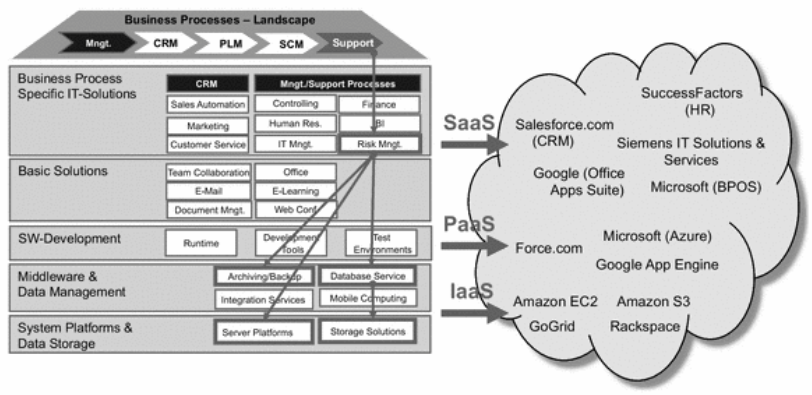
\includegraphics[width=1.0\linewidth]{IaaS_Modelle.png}
	 \captionof{figure}{\small IaaS Modelle \href{http://office.microsoft.com/de-de/business/was-ist-office-365-fur-unternehmen-FX102997580.aspx}{\cite{37}}}
\end{minipage}
\vspace{1em}

Cloud Computing kann in seiner Art nach dem sogenannten technischen Cloud-Stack unterschieden werden. Dies ist ein Schichtenmodell, in dem die obere Schichten auf den unteren aufbauen kann. Jede Schicht kann Anhand ihres Abstraktionsgrades klassifiziert werden:

\begin{compactitem}
\item Schicht 3 - Software as a Service (SaaS):\\
Software, die über eine Cloud-Infrastruktur angeboten wird. Die Bereitstellung, Betreuung und der Betrieb erfolgt gänzlich durch den Anbieter. Eine Abrechnung erfolgt je Softwareaufruf, was den Erwerb der üblichen Software-Lizenz ersetzt. Beispiele hierfür sind \href{http://www.google.com/enterprise/apps/business/}{\textit{Google Apps}} oder \href{http://office.microsoft.com/de-de/business/was-ist-office-365-fur-unternehmen-FX102997580.aspx}{\textit{Microsoft Office 365}}.
\item Schicht 2 - Plattform as a Service (PaaS):\\
Der Anbieter stellt eine verwaltete Cloud-Infrastruktur zur Verfügung, worauf eigene Software bereitgestellt werden kann. Der Kunde erhält zudem eine integrierte Entwicklungs- und Laufzeitumgebung. Eine Abrechnung erfolgt nutzungsabhängig. Zu den Vertretern von PaaS gehören beispielsweise \href{https://cloud.google.com/appengine/}{\textit{Google App Engine}} oder \href{http://azure.microsoft.com/de-de/}{\textit{Microsoft Azure}}.
\item Schicht 1 - Infrastructure as a Service (IaaS):\\
Reine, bedarfsgerechte Nutzung der Rechnerinfrastruktur des Anbieters. Der Anwender muss alles außer der virtuellen Infrastruktur selbst verwalten. Dies bedeutet zwar einen Mehraufwand, bietet aber gleichzeitig eine größtmögliche Skalierbarkeit. Bekannte Anbieter sind \href{https://cloud.google.com/storage/}{\textit{Google Cloud Storage}} oder Amazon Webservices (AWS) mit \href{http://aws.amazon.com/de/}{\textit{Amazon S3 oder Amazon EC2}}. TODO
\end{compactitem}

Im Rahmen dieser Projektarbeit bezieht sich das Konzept auf Infrastructure as a Service (IaaS), worauf nachfolgend im Näheren eingegangen wird.

\subsubsection{IaaS-Typen}
\begin{compactitem}
\item Public IaaS Cloud:\\
Cloud Computing Services für die breite Öffentlichkeit - je Server mehrere unabhängige Nutzer.
\item Private IaaS Cloud:\\
Cloud Computing Services für Unternehmen - je Server ein Unternehmen.
\item Hybrid IaaS Cloud:\\
Cloud Computing Services für Unternehmen - physikalische Server je nach Anwendungsgebiet entweder Public oder Private.
\item Community Cloud:\\
Cloud Computing Services für Unternehmen - Zusammenschluss von Interessensgemeinschaften/Institutionen zur gemeinsamen Nutzung.
\item Personal IaaS Cloud:\\
Cloud Computing Service durch den Anwender selbst.
\end{compactitem}
\pagebreak

\subsubsection{Allgemeine Sicherheitskriterien für IaaS}
\begin{compactitem}
\item Sicherheitsrichtlinien:\\
Jede sicherheitsbewusste Organisation betrachtet und prüft sorgfältig die Einhaltung von Sicherheitsrichtlinien. Die Qualität der Sicherheitspolitik eines IaaS-Anbieters ist ein Indikator dafür, wie dieser für die Verantwortung der Sicherheit einsteht.
\item Unabhängige Sicherheitsbeauftragte:\\
Sicherheitsbeauftragte sollten unabhängig berichten, aber in enger Zusammenarbeit mit technischem Personal des Cloud-Anbieters stehen. Die Verantwortung des Sicherheitspersonals besteht darin, die ständige Sicherheit des Dienstes zu gewährleisten.
\item Upgrades und Patches:\\
Upgrades und Patches sollten in einer zeitgemäßen und sicheren Form umgesetzt werden um Lücken vor der Enthüllung zu beheben und das Sicherheitsniveau stets aufrecht zu erhalten.
\item Untersuchungen:\\
Der Cloud-Anbieter muss regelmäßig Schwachstellenanalysen durchführen und die Infrastruktur nach Auffälligkeiten untersuchen. Alle Funde müssen auf die möglichen Auswirkungen hin bewertet und zeitnah behoben werden.
\item Forensik:\\
Sicherheitsrelevante Protokolle müssen lang genug beibehalten werden, um die Verfügbarkeit für forensische und gesetzliche Anforderungen zu erfüllen. Solche Protokolle tragen zur Ermittlung bei, wie ein Zwischenfall aufgetreten ist und welche Auswirkungen dieser hat.
\item Handhabung von Zwischenfällen:\\
Das Management eines Zwischenfalles und dessen Gegenmaßnahmen sollte darauf ausgelegt sein, den Umfang zu dokumentieren und für den Kunden transparent zu halten. Für den Kunden eines Cloud-Anbieters sind hierbei die Rahmenwerte der Reaktion (Erkennung, Offenlegung, Behebung und Prüfung) für eine weitere Kooperation notwendig.
\item Geschäftskontinuität:\\
RPO (engl. Recovery Point Objective) definiert die Höchstmenge an Datenverlust, welche nach einem entsprechenden Vorfall akzeptabel ist. Ausgedrückt wird dies zusätzlich in Zeit, der Zeit zwischen entsprechendem Verlust und Rückführung zur letzten zuverlässigen Sicherung. RTO (engl. Recovery Time Objective) definiert die Höchstzeitdauer, die für die Wiederherstellung und vollständigen Zugriff auf die Daten akzeptabel ist.
\end{compactitem}
\cite{38}

\subsection{Technische Analyse/Umsetzung}

\subsubsection{Cloud-Anbieter}
Der Markt für Cloud Computing in Form von IaaS befindet sich in einem stetigen Wandel und einer raschen Weiterentwicklung. Aus diesem Grund muss die Wahl des Anbieters sehr sorgfältig und unter Betrachtung aller Gesichtspunkte getroffen werden. Die aktuelle Studie "Magic Quadrant for Cloud Infrastructure as a Service" von Gartner \cite{30} vergleicht die Vorzüge und Nachteile der derzeit angebotenen Produkte unter Betrachtung aller gängigen Anwendungsfälle von IaaS. Hierzu gehören beispielsweise:
\begin{compactitem}
	\item Entwicklung und Testverfahren
	\item Produktionsumfeld (inkl. geschäftskritischer Aufgaben interner und kundenorientierter Anwendungen)
	\item Automatisierung
	\item Wiederherstellung im Sonderfall
	\item Einzelanwendungsfälle und virtuelle Rechenzentren
	\item Entwurfsmuster für native Cloud Anwendungen und Unternehmensanwendungen
\end{compactitem}

\textbf{Magisches Quadrat}
\vspace{1em}
$\;$\\
\begin{minipage}{\linewidth}
	\centering
	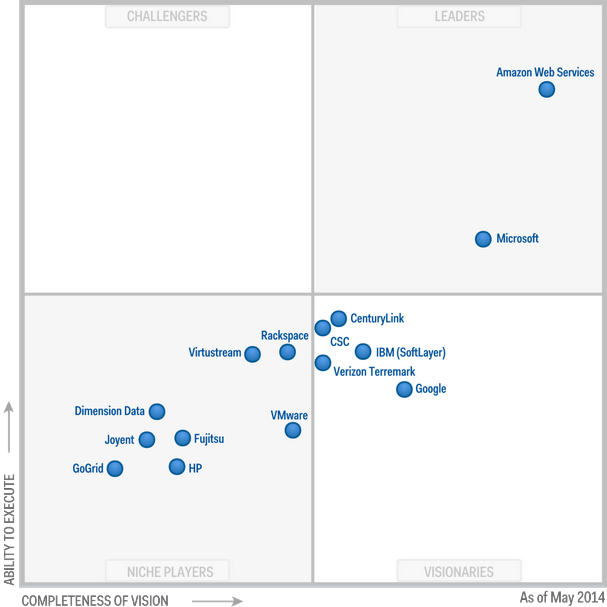
\includegraphics[width=0.7\linewidth]{Gartner_Magic_Square.png}
	\captionof{figure}{\small Magisches Quadrat}
	\label{Gartner}
\end{minipage}
\vspace{1em}

\begin{compactitem}
\item{Marktführer (Leaders):}
\\Der Marktführer-Quadtrant stellt Anbieter dar, die über ein für den strategische Einsatz geeignetes Angebot verfügen und ehrgeizige Ziele verfolgen. Sie sind nicht zwangsläufig der beste Anbieter für spezielle Bedürfnisse und bedienen möglicherweise nicht alle Anwendungsfälle, decken aber ein breites Spektrum davon ab. Marktführer besitzen eine Erfolgsbilanz über erfolgreiche Auslieferung, bedeutende Marktanteile und viele referenzierbare Kunden.
\item{Herausforderer (Challengers):}
\\In dieser Studie befindet sich keiner der Anbieter im Herausforderer-Quadrant. Im Allgemeinen sind Herausforderer in der Lage einige Marktanforderungen zu befriedigen. Sie liefern einen guten Service, welcher auf eine bestimmte Menge von Anwendungsfällen ausgerichtet ist und verfügen über eine Erfolgsbilanz über erfolgreiche Auslieferung. Herausforderer können sich jedoch nicht schnell genug an die Nachfrage auf dem Markt anpassen.
\item{Visionäre (Visionairs):}
\\Visionäre haben eine ehrgeizige Vision von der Zukunft und tätigen erhebliche Investitionen zur Entwicklung von einzigartigen Technologien. Zu ihnen zählen neue Marktteilnehmer oder bestehende Unternehmen, die in einen neuen Markt vorstoßen möchten. Ihre Dienste befinden sich noch im Entstehungsprozess, sie verfügen jedoch über eine Vielzahl an Möglichkeiten zur Entwicklung. Obwohl sie eventuell viele Kunden besitzen, reicht das aktuelle Produkt nicht aus um ein breites Spektrum von Anwendungsfällen zu bedienen.
\item{Nischenspieler (Niche Players):}
\\Nischenspieler sind womöglich ausgezeichnete Anbieter für Anwendungsfälle auf die sie sich spezialisiert haben, können aber bei weitem nicht alle Anwendungsfälle abdecken. Sie können in diesen Markt neu eingetreten sein oder noch nicht über ausreichend signifikante Marktanteile verfügen. Nischenspieler können Marktführer in einem Gebiet abseits von IaaS sein, befinden sich aber zum aktuellen Zeitpunkt für Cloud-IaaS in relativ frühen Stadien. Je speziefischer die Bedürfnisse, desto wahrscheinlicher ist das passende Produkt in diesem Quadranten zu finden.
\end{compactitem}

\textbf{Entscheidungsgrundlage Cloud-Anbieter}\\
In Abbildung \ref{Gartner} ist ersichtlich, dass die Top-Unternehmen Amazon (Amazon Web Services) und Microsoft (Microsoft Infrastructure Services) bei den aktuellen Marktführern einzuordnen sind, während sich Google mit seinem IaaS-Angebot Google Cloud Storage im Quadrant der Visionäre befindet.

Die Strategie der Google Cloud Plattform basiert auf dem Konzept anderen Unternehmen eine Leistungsfähigkeit anzubieten, wie Google sie selbst verwendet. Dies wird durch Nutzung der innovativen internen technischen Möglichkeiten erreicht. Obwohl Google erst im Dezember 2013 in den IaaS-Markt vorgedrungen ist (seit 2008 Google App Engine als PaaS), befindet sich die angebotene Lösung bereits unter den Visionären. Das liegt unter anderem daran, dass sich Google auf seine Fähigkeiten beschränkt, anstatt diese von Grund auf neu zu strukturieren. Daher wird es auf lange Sicht in der Lage sein das Angebot schneller als seine Konkurrenten voranzubringen. Google verfügt über eine umfassende Vision und ausreichend Erfahrung darüber, wie native Cloud-Anwendungen über einen Lebenszyklus hinweg entwickelt und verwaltet werden. Die Vorstellung von fließenden Grenzen zwischen IaaS und PaaS wird Anwendern in absehbarer Zeit einen Kompromiss zwischen Kontrolle und automatisierter Verwaltung bieten. Die gesamte Unternehmung Google verfügt über eine Vielzahl von Rechenzentren, enorme infrastrukturelle Kapazitäten und ein eigenes globales Hochleistungsnetzwerk. Da der IaaS-Zweig Google Compute Engine (GCE) lediglich geringe Mehrkosten für Google darstellt, kann es den Preis trotz hoher Leistungsfähigkeit aggressiv gestalten. Dennoch wird sich Google nicht durch den Preis, sondern durch seine Plattform und zusätzliche Verwaltungsfunktionen von den anderen IaaS-Anbietern unterscheiden. Aktuell ist Google Cloud Storage jedoch ein relativ neues Produkt, sodass noch keine operative Erfolgsbilanz gezogen werden kann. Hinzu kommen kleinere Störungen bis zur Freigabe der allgemeinen Verfügbarkeit von GCE. Eine der größten Herausforderungen besteht darin, das Vertrauen der Unternehmen zu gewinnen und den Support auszubauen. Allerdings wird Google bereits heute als künftiger Marktführer für IaaS wahrgenommen, nicht zuletzt wegen der gewohnten Unterstützung durch Software-Unternehmen und Entwickler. Diesen Vorteil konnten wir uns im Rahmen der Projektarbeit zunutze machen und auf Entwicklungsmöglichkeiten von Google, bspw. durch die Verwendung der Schnittstelle gsutil, zurückgreifen. Da das Ziel dieser Arbeit ebenfalls in einem visionären Quadranten einzuordnen wäre, haben wir uns für Google Cloud Storage und gegen Amazon Web Services und Microsoft Infrastructure Services entschieden.

\subsubsection{Java}\label{JavaV}
Die Anwendung zur sicheren Speicherung in der Cloud wurde komplett in Java in der Version 1.7 implementiert. Der Ursprung von Java liegt in den frühen 90er Jahren, als ein Team um James Gosling (genannt das Green Team) bei Sun Microsystems damit began eine der ersten plattformunabhängigen Programmiersprachen zu entwickeln. Sie sollte die Computerwelt revolutionieren indem sie die Grenzen zwischen den Systemen, die damals noch deutlicher waren als heute, verwischt. Heute gehört die gesamte Java Technologie der Oracle-Gruppe, die Sun Microsystems im Januar 2010 kaufte.\\
Die Java Technologie, welche die Plattformunabhängigkeit zur Verfügung stellt, besteht im Kern aus drei Teilen:
\begin{compactitem}
	\item JDK: Java Development Kit
	\item Java: Die Programmiersprache
	\item JRE: Java Runtime Environment
\end{compactitem}

Das \textbf{Java Development Kit} ist das Entwicklungswerkzeug mit welchem Java Anwendungen erstellt werden können. Seit 2006 wird es von Sun Microsystems unter der Gnu Public License mit einer sog. Linking Exception (Ausnahmegenehmigung für das Linken einer Programmbibliothek) veröffentlicht und mittlerweile wird es von einer OpenSource Commuinity in enger Zusammenarbeit mit Firmen wie IBM und Apple als OpenJDK in einer freien Version weiterentwickelt. Es besteht hauptsächlich aus Bibliotheken, sowie dem Java Compiler \textbf{Javac} mit dem aus Java Code der sog. \textbf{Java-Bytecode} erzeugt werden kann.\\
Die Programmiersprache \textbf{Java} ist eng mit C++ verwandt und strikt Objekt orientiert. Das besondere an Java sind außerdem eine Vielzahl an Bibliotheken, die vom JDK direkt mitgeliefert, und (als es noch ausschließlich Sun gehörte) von Sun Microsystems gewartet werden. Hierdurch können viele Standardaufgaben, die bei der Entwicklung anfallen, direkt mit einer Java Bibliothek gelöst werden, ohne dass diese Funktionalitäten erst entwickelt oder weite externe Bibliotheken eingebunden werden müssten, die dann weitere Lizenzen erfordern oder zweifelhaften Ursprungs sind.\\
Das \textbf{Java Runtime Environment} ist die Besonderheit der Java Technologie, welche den plattformunabhängigen Betrieb der Java Anwendungen erst ermöglicht. Das  JRE nimmt keinen üblichen Maschinencode entgegen, der Prozessessorgebunden wäre, und damit nur auf bestimmten Architekturen laufen könnte, sondern \textbf{Java-Bytecode}. Dieser Bytecode besteht auch aus Prozessoranweisungen, allerdings für den Prozessor der virtuellen Maschine, welche das JRE zur Verfügung stellt. Darin besteht der Kern der Plattformunabhängigkeit: Wurde einmal ein JRE für die betreffende Architektur und das Betriebssystem entwickelt, sind Java Anwendungen auf diesem lauffähig, solange sie sich strikt an Java und seine Bibliotheken halten.\\
Diese Besonderheit ist auch der Grund, aus dem die Wahl der Programmiersprache zu Beginn des Projektes auf Java fiel. Zum Einen kann die Software ohne Portierungsaufwand auf allen gängingen Betriebssystemen verwendet werden, zum Anderen entfällt ein großer Teil des Entwicklungsaufwandes für Funktionalitäten die nicht dem Kern der Software dienen, wie ein grafisches Interface oder der Umgang mit Dateien und Ordnern. Dadurch lässt sich mehr Zeit auf die eigentlichen Kernfunktionen wie Verschlüsselung und Cloudanbindung,  sowie das zugrunde liegende Sicherheitskonzept verwenden. \cite{1}\cite{2}\\\cite{3}

\subsubsection{Schnittstelle Google Cloud Storage: gsutil}
\textbf{gsutil} \cite{32} ist eine Python-Anwendung, welche einen konsolenbasierten Zugriff der gängigen Betriebssysteme Linux/Unix, Mac OS oder Windows auf Google Cloud Storage ermöglicht. Voraussetzung ist ein installiertes Python in der Version 2.6.x oder 2.7.x,  Python 3.x ist dazu derzeit inkompatibel. Dabei nutzt gsutil die Notation der Standardbefehle von Linux, welche direkt in einer Konsole oder durch eine Anwendung aufgerufen werden können. Damit gsutil als Schnittstelle zum eigenen Google Cloud Storage verwendet werden kann, muss dieses initial durch einen Authentifizierungscode mit dem zugehörigen Account verknüpft werden. TODO :BOTO Nachfolgend sind die für das Projekt relevanten Befehle aufgelistet (ein Ausführen von gsutil mit einem Python-Interpreter und eine korrekte Authentifizierung ist vorausgesetzt): TODO BUCKET

\begin{compactitem}
	\item Auflisten: \textbf{ls}\\
	gsutil ls [Optionen] gs://\textless Bucket\textgreater
	\item Kopieren: \textbf{cp}\\
	Upload: gsutil cp [Optionen] \textless Quellpfad lokaler Datei\textgreater~gs://\textless Bucket\textgreater\\
	Download:  gsutil cp [Optionen] gs://\textless Bucket\textgreater/\textless Dateiname\textgreater~\textless Zielpfad lokaler Datei\textgreater
	\item Entfernen: \textbf{rm}\\
	gsutil rm [Optionen] gs://\textless Bucket\textgreater /\textless Dateiname\textgreater
\end{compactitem}

Desweiteren verarbeitet gsutil Befehle für das Erstellen und Löschen von Buckets, Verschieben, Umbenennen und Editieren von Objekten sowie zur Rechteverwaltung.

Neben der Schnittstelle gsutil verfügt Google Cloud Storage über eine \textbf{XML API} für HTTP-Anfragen von Web-Services, eine \textbf{JSON API} in Version v1 und weitere \textbf{Cloud Storage Tools}.TODO warum gsutil, WEBSOCKET ETC\\

\subsubsection{Eclipse IDE for Java Developers}
Eclipse ist eine OpenSource Entwicklungsumgebung zur gestützten Entwicklung von Software. Die IDE for Java Developers beinhaltet zusätzlich Pakete und Tools, die eine Programmierung in der Programmierhochsprache Java erleichtert. Interessant hierbei ist, das Eclipse selbst für Java und auch in Java Entwickelt wurde. Es ist also genau so vielseitig nutzbar wie die Anwendungen die damit entwickelt werden. Durch Plugins kann die Funktionalität von Enclipse erweitert werden, etwa um UML Diagramme aus Code oder umgekehrt aus UML Diagrammen Code zu erzeugen, oder um die Entwicklung in anderen Sprachen zu ermöglichen. Im Zuge dieses Projekts wurde Eclipse in der Version \textbf{Kepler Service Release 2}, \textbf{Build id: 20140224-0627}, verwendet.

\subsubsection{Versionsverwaltung: git}
\textbf{git} ist eine Software unter der OpenSource-Lizenz GNU GPLv2, welche zur verteilten Versionsverwaltung von Dateien eingesetzt wird. Seinen Ursprung fand git in der Verwaltung von Quellcode zur Entwicklung des Linux-Kernels. In diesem Projekt fand Version 2.1.2, unter Einsatz von Atlassian SourceTree TODO LINK als Interface, Verwendung. Dies machte eine gleichzeitige, standortunabhängige Entwicklung und Synchronisierung von Änderungen des Prototyps möglich. \cite{31}

\subsubsection{Kryptographische Verfahren}
\textbf{AES}\\
AES (Advanced Encryption Standard) ist ein Kryptosystem, welches im Zuge einer 1997 bekannt gegebenen Ausschreibung des US-Amerikanischen Handelsministeriums Standardisiert wurde. Es hat die mittlerweile als unsicher geltenden DES bzw. 3DES Kryptosysteme abgelöst, gilt heute als Standard der symmetrischen Verschlüsselung und als für viele Jahre sicher. Es gibt ihn in den Varianten AES-128, AES-192 und AES-256, wobei die Zahlen sich auf die jeweils verwendete Schlüssellänge in Bit beziehen. Der verwendete Algorithmus ist der Rijndael von Vincent Rijmen und Joan Daemen. Unter anderem wird er von der NASA und der US-Amerikanischen Regierung verwendet und ist Teil der Standards WPA2, SSH, IPSec, SSL und vielen mehr. Außerdem ist er in jedem größeren Betriebssystem an der einen oder anderen Stelle implementiert. Diese sehr hohe Verbreitung ist vor allem auf seine Einfachheit, der Möglichkeit ihn in Hardware zu implementieren, der mathematischen Eleganz, dem geringen Rechenaufwand und nicht zuletzt dem offenen Ausschreibungsverfahren geschuldet. Grade die Besonderheit, dass dieser Standard der US-Amerikaner offen liegt, von jedem selbst implementiert werden kann, nicht übernommen werden muss und in einem äußerst transparenten Verfahren ausgeschrieben und ausgewählt wurde, wird bis heute gelobt und ist Hauptgrund für das in AES gesetzte Vertrauen. Grundsätzlich ist AES eine symmetrische Blockchiffre. Es arbeitet also bei Ver- und Entschlüsselung mit den selben Schlüsseln. Außerdem werden die Nutzdaten in 16 Byte Blöcke geteilt, welche getrennt verschlüsselt werden. Die Blockgröße ist im Gegensatz zur Schlüssellänge nicht variierbar. Der Algorithmus sieht die Möglichkeit zwar vor, sie wurde jedoch nicht im AES standardisiert.
\\\textbf{Funktionsweise}\\ 
Wird ein 16 Byte Block mit dem AES verschlüsselt, wird dieser Block zunächst in eine Tabelle mit vier Zeilen und vier Spalten geschrieben, wobei jedes Feld der Tabelle ein Byte enthält. Nun werden die einzelnen Felder mehrfach mit unterschiedlichen Teilen des erweiterten Schlüssels chiffriert, wobei über die Schlüssellänge k definiert wird, wieviele dieser Verschlüsselungsrunden r es gibt (Fall AES-128: 10 Runden). Aus dem Schlüssel k werden nun (r + 1) Rundenschlüsselgeneriert indem k in eine weitere Tabelle mit (im Fall AES-128) vier Zeilen und 44 Spalten eingetragen wird. Nachdem der Schlüssel in die ersten Byte-großen Felder der Tabelle gelegt wurde, werden die restlichen rekursiv nach bestimmten Rotations- und Berechnungsverfahren gefüllt. Nach dieser Vorbereitung werden die Nutzdaten in der ersten Tabelle jetzt in mehreren Runden zunächst mit dem jeweiligen Rundenschlüssel XOR-Verknüpft. Danach werden die einzenen Felder der Tabelle wieder nach festgelegten Prinzipien innerhalb ihrer Spalte nach links verschoben. Links herausfallende Werte werden rechts wieder in die Tabelle eingefügt, es wird also rotiert. Nun werden die einzelnen Werte innerhalb der Spalten nach definierten Verrechnungssystemen (Spaltenwert * [1|2|3] modulo [irreduzibles Polynom] | innerhalb des Glasios-Körpers, anschließend untereinader XOR-Verknüpft) vermischt. Nachdem dieses Verfahren (Verknüpfung mit dem Rundenschlüssel, rotieren der Zeilen, vermischen der Spalten) r-Mal ausgeführt wurde ist die Verschlüsselung abgeschlossen. Die Entschlüsselung durchläuft, wie bei allen symmetrischen Kryptosystemen, exakt die selben Schritte in umgekehrter Reihenfolge. \cite{4}\cite{5}\\
\\\textbf{Counter Mode}\\
Für Blockchiffren wurden im Laufe der Jahre verschiedene sog. Betriebsmodi entwickelt. Ein Betriebsmodus stellt die Art und Weise da in der eine Blockchiffre verwendet wird. Mit der Verwendung von Betriebsmodi ist es unter anderem möglich Blockchiffren   als   Stromchiffren   zu   verwenden,   Nachrichten   mit   mehrfacher   Blocklänge   zu   verschlüsseln   oder selbstsynchronisierende Chiffren zu erzeugen. Einer dieser Betriebsmodi ist der sog. Counter Mode.
Im Counter Mode wird nicht der Klartext selbst mittels Algorithmus und Schlüssels chiffriert sondern es wird mittels eines (im besten Fall zufällig) gewählten Initialisierungsvektor (Nonce, number only used once) und einem Zähler (Counter) eine Bytefolge in Blocklänge gebildet. Diese wird dann mittels des Schlüssels chiffriert und per XOR Operation mit einem der Blocklänge entsprechen Teil des Klartextes verknüpft. Danach wird der Zähler um eins erhöht und auf die Selbe Weise mit dem Rest der Nachricht fortgefahren. Wichtig zu verstehen ist hierbei, dass der Initialisierungsvektor nicht Teil des Geheimnisses ist (welches ausschließlich der Schlüssel darstellt, siehe Kerckhoffs‘ Prinzip), sondern offen übertragen werden kann. Es dient ausschließlich der Diversifikation gleicher Klartexte und dem Auffüllen einer Blocklänge. Durch den Counter Mode ist es möglich, Blockchiffren als Stromchiffren zu betreiben, da Klartexte beliebiger Länge mit den erzeugten Chiffratbytes bitweise verknüpft werden können. Vorteil bei diesem Modus ist auch, dass Chiffrate im Voraus errechnet werden können, wodurch sich unter Umständen Zeitvorteile ergeben. Fehlerhaft übertragene Bits werden eins zu eins fehlerhaft entschlüsselt, weitere Teile der Nachricht sind nicht betroffen. \cite{6}\cite{7}\\
\\\textbf{Kryptographische Hashfunktionen: SHA2-256}\\
SHA (Secure Hash Algorithm) ist eben so wie der AES eine Standardisierung. In diesem Falle allerdings die Standardisierung eines sicheren Hash Algorithmus. 

Ein sicherer Hash Algorithmus ist in erster Linie eine Hashing Funktion wie jede Andere, also ein Algorithmus, der Prüfsummen auf Eingabewerte beliebiger Länge berechnet. Prüfsummen fanden schon vor der Kryptographie Einsatz in der Informatik, vor allem um die korrekte Übertragung von Daten zu gewährleisten. Ein gutes Beispiel hierfür bietet der CRC (Cyclic Redundancy Check). Wenn aus einem Bitstrom mittels CRC eine Prüfsumme brechnet wurde, kann anhand dieser nach der Übertragung der Daten relativ sicher festgestellt werden, ob alle Daten korrekt übertragen wurden, da der CRC Wert sich durch kleinste Veränderungen im Bitstrom stark verändert. Im Falle der kryptogephischen Hash Funktion ist diese Eigenschaft eben so wichtig, allerdings kommen  in diesem Umfeld weitere Anforderungen hinzu: Eine kryptographische Hash Funktion sollte eine Einwegfunktion sein. Das bedeutet, dass es nicht möglich sein darf, aus einem Berechneten Hashwert die ursprüglichen Daten zu rekonstruieren. Die meisten Hash Funktionen stellen dies sicher, indem der Hashwert kürzer als die Eingabedaten ist. Durch diese Kompression ist es nicht mehr möglich die ursprünglichen Daten zu ermitteln. Eine weitere Anforderung ist, dass eine kryptographische Hashfunktion kollisionsresistent sein muss. Bei einer kollisionsresistenten Hashfunktion ist es nicht möglich in effektiver Zeit einen zwei unterschiedliche Datenströme zu berechnen die den selben Hashwert erzeugen. TODO BSI Aus dieser Anforderung ergibt sich auch, dass es nicht möglich ist einen Datenstrom derart zu bearbeiten, dass er einen gewünschten Hash produziert. Diese Anforderungen erfüllt CRC nicht, dafür aber kryptographische Hashfunktionen wie die in SHA standardisierten. Dagegen sind diese meist deutlich komplexer (rechenintensiver) und die erzeugten Hashes länger. Der eigentliche Sinn und Zweck von kryptographischen Hashfunktionen liegt vor allem in zwei Anwendungsfällen:
\\\textbf{Sicherstellung von Integrität}\\
Um die Integrität eines übertragenen Bitstroms zu garantieren, kann der Hashwert zusätzlich sicher mit übertragen werden (überlicherweise asymmetrisch verschlüsselt). Nach dem Erhalt der Nachricht, kann der Empfänger anhand des Hashes überprüfen ob sie unverändert übertragen wurde. Hier liegt auch der Grund der Kollisionssicherheit: Es ist effektiv nicht möglich eine neue sinnvolle Nachricht mit einem manipulierten Inhalt zu erzeugen, die den selben Hash aufweist.
\\\textbf{Beweis: Geheimnisbesitz}\\\label{KryptV}
Will eine Person einer Anderen beweisen im Besitz eines Geheimnisses zu sein, vertraut aber der Übertragung nicht und möchte es daher nicht preisgeben, kann sie einen sog. Salt (Eng. Salz, von versalzen) erzeugen und diesen mit dem Geheimnis zusammen hashen. Dieser Hash inklusive des Salt wird verschickt und der Empfänger kann seinerseits das Geheimnis und den Salt hashen. Ist der anderen Person das Geheimnis bekannt, müssen die Hashes sich gleichen. Der Salt dient in diesem Fall der Sicherstellung, dass ein eventueller Angreifer den Hash des reinen Passwortes nicht aufzeichnen kann und sich mit dem Besitz des Hashes als Kenner des Geheimnisses ausgibt. Außerdem verhindert der Salt, dass Passwortlisten (sog. Rainbowtables) von gehashten Geheimnissen (in diesem Fall : Passwörtern) vorrausberechnet und mit gestohlenen Hashes abgeglichen werden können. Dieses Verfahren wird zum Beispiel verwendet, wenn Server Passwörter für den Login speichern. So müssen sie die Passwörter nicht im Klartext speichern, und der Schaden bei einem Einbruch kann minimiert werden. TODO

SHA2 ist der Nachfolger von SHA1 und ermöglicht die Erzeugung von sicheren Hashes von 224, 256, 384 oder 512 Bit Länge. Der Algorithmus dieser verschiedenen Versionen ist grundsätzlich immer der selbe, allerdings unterscheiden sich die Anzahl der berechneten Runden und die Länge der Initialwerte. Zum Teil (256 zu 224) wird auch einfach der letzte Teil der Ausgabe ignoriert und damit eine geringere Länge des Hashwertes erreicht. \cite{8}\cite{9}\cite{10}\\
\pagebreak



% ----------------------------------------------------------------------------------------------------------
% Ergebnisse
% ----------------------------------------------------------------------------------------------------------
\section{Ergebnisse}
TODO Einleitung
\subsection{Architektur}
Der Software zugrunde liegt eine Architektur, die an das Model-View-Control Entwurfsmuster angelehnt ist. Sie unterteilt sich in drei packages (Abgrenzung von Programmteilen in Java) sowie zwei subpackages (packages, die in anderen enthalten sind). Im Folgenden werden diese sowie die enthaltenen Klassen näher skizziert. Eine genaue Auflistung der Methoden und Klassenvaiablen kann den UML Diagrammen bzw. der Dokumentation entnommen werden.

\textbf{Package: control}\\
Das package control enthält die Programmlogik, hierzu gehören Ver- und Entschlüsselung, Nutzerverwaltung und Koordination der Datei-Informationen.\\
\textbf{Klasse: Main}\\
Die Klasse Main stellt das Herz der Applikation dar: In ihr liegen applikationsweit verwendete Definitionen (public static final Variablen) und Methoden die von den Views aus aufgerufen werden um auf Benutzerinteraktionen zu reagieren. Die meisten anderen Klassen werden hier instanziert, die temporären Benutzerinformationen hinterlegt und mit get() und set() Methonden für andere Module nutzbar gemacht. Sie stellt also den Knotenpunkt dar, der die Module der Applikation verbindet. Main ist an der Programmlogik selbst nur in Form des Programmstartes und der Delegation anderer Aufrufe beteiligt. Kalkulationen oder Dateioperationen finden hier nicht statt. Sie ist mit dem Singelton Entwurfsmuster implementiert. Auf diese Weise ist sichergestellt, dass alle Programmteile auf die selbe Instanz von Main zugreifen, ohne dass eine entsprechende Referenz an die anderen Klassen übergeben werden müsste.\\
\textbf{Klasse: FileListHandler}\\
Auch der FileListHandler ist ein Singleton, kommt also applikationsweit nur in einer Instanz vor und wird von verschiedenen Programmteilen direkt aufgerufen. Im Kern besteht er aus einem Vector aus InformationContainer Instanzen (siehe Package model - InformationContainer), sie ist also das temporäre (während des Programmablaufes) Speichermodul für Informationen über die in der Cloud liegenden Dateien. Zusätzlich besitzt sie Methoden für Operationen auf diesem Vector, etwa neue Dateien hinzuzufügen oder aber Dateien anhand bestimmter Schlüssel zurück zu geben.\\
\textbf{Klasse: SettingsFileHandler}\\
Der SettingsFileHandler verwaltet die Datei settings.cfg in der Informationen über in der Applikation registrierte Benutzer gespeichert sind. Er erzeugt sie bei Bedarf, liest eine bestehende ein und macht die Benutzerinformationen anderen Programmteilen zugänglich oder schreibt neue Benutzer hinein.\\
\textbf{Klasse: SystemInformationCollector}\\
Der SystemInformationCollector sammelt, wie der Name suggeriert, Informationen über das System auf dem die Applikation gestartet wird. Zurzeit ist dies ausschließlich die Information über das zugrunde liegende Betriebssystem, es sind jedoch für die Zukunft weitere Informationen vorgesehen, etwa die Anzahl der Prozessorkerne um mittels Verteilung der Rechenlast schneller zu ver- und entschlüsseln. TODO Discussion\\
\textbf{Klasse: SystemPathCollector}\\
Der SystemPathCollector macht anderen Modulen Informationen darüber zugänglich, wo sich weitere, für die Applikation notwendige, Programme befinden. Zurzeit sind dies Python und Gsutil.\\
\textbf{Klasse: ThreadInstanceCreator}\\
Der ThreadInstanceCreator ist für das Threading zuständig. Im Laufe der Entwicklung stellte sich heraus, dass vor allem ver- und entschlüsselt, sowie der Up- und Download großer Dateien den Programmablauf erheblich behindern, daher war es notwendig diese Operationen in einen weiteren Prozess auszulagern. Dies wird von ThreadInstanceCreator übernommen. Für jede neue Verschlüsselungs-, Up- bzw. Download- und Entschlüsselungsoperation wird eine neue Instanz dieser Klasse als neuer Thread erzeugt. Möglich wird dies über das von Java zur Verfügung gestellte Interface Runnable, welches die Klasse implementiert (implements). Eine neue Instanz bekommt im Konstruktor einen InformationContainer sowie einen Befehl (enum), wie dieser zu verarbeiten ist, übergeben und arbeitet Ver- bzw Entschlüsselung und Up- und Download selbstständig ab.\\
\textbf{Subpackage: util}\\
Das subpackage util gehört zum controller und besitzt Methoden die softwareweit unabhängig sind, also keine initialisierten Instanzen benötigen, etwa weil keine Klassenvariablen zur Speicherung von Informationen notwendig sind. Alle Methoden dieser Klassen sind statisch und können zu jeder Zeit von jedem Programmteil verwendet werden. Unter anderem liegen hier die Verschlüsselungsfunktionen sowie Hilfsfunktionen zur Umwandlung von Werten. \\
\textbf{Klasse: CryptToolbox}\\
Die CryptToolbox bietet Ver-/Entschlüsselung von Dateien oder Bytearrays, Hashing sowie die Generierung von kryptographisch sicheren Zufallszahlen. Auch werden hier die ThreadInstanceCreator Instanzen erzeugt, die dann Funktionen der CryptToolbox verwenden.\\
\textbf{Klasse: SupportFunctions}\\
Eine Hilfslasse um Integer in Bytes zu konvertiert sowie, zur Erleichterung des Debuggings, Bytearrays auf der Konsole auszugeben.\\

\textbf{Package: model}\\
Das package model ist für die Daten selbst zuständig, es definiert in welcher Weise Informationen gespeichert und, nach Beendigung des Programmes, lokal im Speicher des Computers abgelegt werden.\\
\textbf{Klasse: InformationContainer}\\
Ein InformationContainer stellt in der Programmlogik eine in der Cloud liegende Datei dar. Er besitzt Klassenvaribalen in denen Name, Schlüssel, Dateipfad und weitere Informationen gespeichert sind sowie get() und set() Funktionen um auf und mit diesen Informationen zu arbeiten.\\
\textbf{Klasse: InformationContainerStorer}\\
Der InformationContainerStorer verarbeitet die Speicherung bei Beendigung der Applikation sowie das Laden der InformationContainer nach Programmstart. Er verwaltet die entsprechende Datei (state.cfg) und stößt an, dass die  InformationContainer vor dem Speichern in Bytearrays umgewandelt und mittels des Benutzerpasswortes verschlüsselt werden.\\
\textbf{Subpackage: cc}\\
Das subpackage cc gehört zum model und verwaltet die Speicherung der Daten in der Cloud. Darin wird das Interface für die Schnittstelle zu Cloudspeichern definiert. In diesem Prototyp ist dies gsutil zur Anbindung von Google Cloud Storage.\\
\textbf{Interface: CloudConnector}\\
Das Interface CloudConnector definiert, wie eine Schnittstelle zu einem Cloudanbieter aufgebaut sein muss, also welche Methoden sie besitzen muss und welche Übergabeparameter bzw. Rückgabewerte diese haben.\\
\textbf{Klasse: CloudConnectorGoogleGsutil}\\
Der CloudConnectorGoogleGsutil ist eine Implementierung des Interfaces CloudConnector zur Anbindung des Google Cloud Storage mittels der Python Schnittstelle gsutil und stellt die in CloudConnector definierten Methoden für Operation auf dem Cloudspeicher bereit.\\

\textbf{Package: view}\\
Das package view enhält alle Teile des grafischen Interfaces. In diesem werden alle Fenster definiert. Die views verfügen über lediglich zwei Schnittstellen zur resltichen Applikation: Die Main Klasse, welche Aktionen (klicks) auf den Views entgegen nimmt und daraufhin andere Programmteile steuert, sowie die Klasse FileListHandler, welche dem MainWindow die in der Tabelle aufgelisteten Informationen (in der Cloud befindliche Dateien, InformationContainer) liefert. Eine genaue Beschreibung, wie das GUI aufgebaut ist, befindet sich in \ref{GUIV} GUI und Funktionalitäten\\
\textbf{Klasse: MainWindow}\\
Das MainWindow ist die Hauptoberfläche der Apllikation. Hier wird eine Liste der in der Cloud befindlichen Dateien angezeigt, es können weitere zum Upload ausgewählt oder aus der Cloud gedownloaded bzw. gelöscht werden.\\
\textbf{Klasse: CreateAccountWindow}\\
Das CreateAccountWindow erscheint, wenn der Benutzer entweder noch keinen Account angelegt hat, oder aber wenn die Schaltfläche Create im LoginWindow ausgewählt wird. Hier muss vom Benutzer sein gewünschter Nutzername, sein Passwort sowie eine Wiederholung, zur Vorbeugung eines Tippfehlers, eingeben werden.\\
\textbf{Klasse: DeleteWindow}\\
Das DeleteWindow erscheint, wenn die Applikation beim Start feststellt, dass im lokalen Speicher InformationContainer hinterlegt sind, die kein Pendant mehr in der Cloud besitzen. Dies kann geschehen, wenn sie manuell per Webinterface gelöscht wurden, oder aber der Upload fehl schlug. Der Benutzer sieht hier um welche Datei es sich handelt (Klarname, ID in der Cloud) und kann selbst enscheiden ob der InformationContainer zur Sicherheit behalten werden sollte, oder entfert werden kann.\\
\textbf{Klasse: LoginWindow}\\
Das LoginWindow fordert den Benutzer auf seine Nutzerdaten einzugeben um sich in der Applikation einzuloggen. Dies sind sein Nutzername, das dazugehörige Passwort sowie der Bucket auf dem der Nutzer arbeiten möchte. Dies ist zurzeit sehr Google Storage spezifisch, allerdings ist die Applikation aus dem Grund modularisiert aufgebaut. Hier können später weitere Cloudanbieter mit alternativen LoginWindows angebunden werden.\\
\textbf{Klasse: NonEditableJTable}\\
Die NonEditableJTable ist eine Hilfsklasse. Sie erbt vom DefaultTableModel (Javaklasse die die Methoden von JTables definiert) und überschreibt die Funktion isCellEditable(int row, int column), sodass sie immer false zurück gibt. Im MainWindow erhält die angezeigte Tabelle dieses Model, damit der Benutzer die Tabelle nicht manuell bearbeiten kann, was zurzeit in der Applikation keinen Sinn machen würde und Fehler im Programmablauf erzeugen könnte.\\
\textbf{Klasse: NotificationWindow}\\
Das NotificationWindow wird angezeigt, wenn der Benutzer die Menüpunkte Help oder About in der Menüleiste im MainWindow betätigt. Entsprechend zeigt das NotificationWindow mit der Help Option eine Erklärung zur Bedienung der Applikation, wenn About ausgewählt wurde stehen dort Informationen über Entwickler und Version.


\subsubsection{UML-Diagramme}
Die UML Diagramme befinden sich im digitalen Anhang, Ordner UML. In der Datei ClassRelations.jpg findet sich eine Übersicht aller Klassen und deren Beziehungen zu einander. Attribute und Methoden wurden hier weg gelassen, da diese der Übersichtlichkeit abträglich wären. Des Weiteren gibt es für jedes package bzw. subpackage ein weiteres UML mit den jeweiligen Klassen, deren Beziehungen sowie Attributen und Methoden. Genauere Beschreibungen der einzelnen Methoden, Klassen und Attributen finden sich in der Dokumentation im Ordner Projektdokumentation im digitalen Anhang. TODO

\pagebreak

\subsubsection{Anwendungsfälle}
\vspace{1em}
$\;$\\
\begin{minipage}{\linewidth}
	\centering
	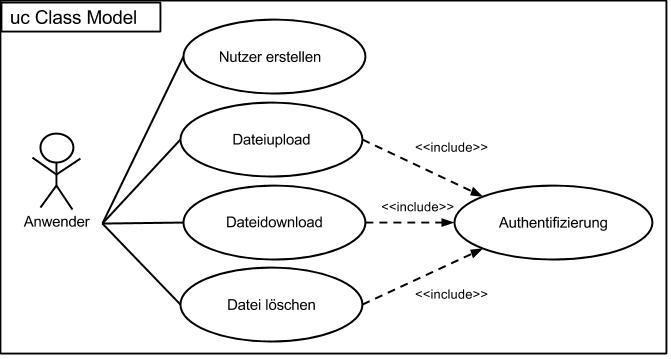
\includegraphics[width=0.8\linewidth]{UseCase.jpg}
	 \captionof{figure}{\small Anwendungsfalldiagramm}
\end{minipage}
\vspace{1em}

\textbf{AF-001 Nutzer erstellen:}
\begin{table}[!h]
	\centering
	\begin{tabular}{|l|l|}
		\hline
		Nummer & AF-001\\
		\hline
		Name & Nutzer erstellen\\
		\hline
		Akteure & Anwender\\
		\hline
		Auslöser & Anwender möchte einen Benutzer anlegen\\
		\hline
		Vorbedingung & Programm zeigte den Login-Dialog, Anwender hat \\ &  Create ausgewählt\\
		\hline
		Nachbedingung/Ziel & Ein neuer Benutzer wurde angelegt \\
		\hline
		Nachbedingung im Sonderfall & Es wurde kein Benutzer erstellt \\ & Erneute Aufforderung zur Dateneingabe\\
		\hline
		Normalablauf & 1. Anwender strartet Programm \\ & 2. Anwender wählt Create im Login-Fenster\\ & 3. Anwender gibt Benutzername ein \\ & 4. Anwender gibt Passwort ein \\ & 5. Anwender bestätigt das Passwort durch zweite\\ &Eingabe\\& 6. Benutzer wurde angelegt\\& 7. Login-Fenster wird angezeigt \\
		\hline
		Sonderfälle & 3a. Anwender gibt nicht erlaubten Benutzernamen ein \\ & 4a. Anwender gibt nicht erlaubtes Passwort ein \\& 5a. Anwender gibt nicht das identische Passwort ein\\& 6a. Benutzer konnte nicht angelegt werden \\& 7a. Create-Fenster wird erneut angezeigt\\
		\hline
	\end{tabular}
	\caption{AF-001 Nutzer erstellen}
	\label{tab:AF-001 Nutzer erstellen}
\end{table}

\textbf{AF-002 Authentifizierung:}
\begin{table}[!h]
	\centering
	\begin{tabular}{|l|l|}
		\hline
		Nummer & AF-002\\
		\hline
		Name & Authentifizierung\\
		\hline
		Akteure & Anwender\\
		\hline
		Auslöser & Anwender möchte sich anmelden\\
		\hline
		Vorbedingung & Programm zeigt den Login-Dialog, Anwender ist im \\ &  Cloud-System registriert und zum Zugriff berechtigt\\
		\hline
		Nachbedingung/Ziel & Erfolgreiche Anmeldung am Cloud-System \\
		\hline
		Nachbedingung im Sonderfall & Zugriff verweigtert\\ & Erneute Aufforderung zur Anmeldung\\
		\hline
		Normalablauf & 1. Anwender strartet Programm \\ & 2. Anwender gibt Benutzername ein \\ & 3. Anwender gibt Passwort ein \\ & 4. Anwender gibt Bucket an \\ &5. Zugangsdaten werden überprüft \\ & 6. Dateiübersicht wird angezeigt \\
		\hline
		Sonderfälle & 2a. Anwender gibt falschen Benutzernamen ein \\ & 3a. Anwender gibt falsches Passwort ein \\& 4a. Anwender gibt nicht gestatteten Bucketnamen an\\ & 5a. Erneutes Laden der Loginmaske\\
		\hline
	\end{tabular}
	\caption{AF-002 Authentifizierung}
	\label{tab:AF-002 Authentifizierung}
\end{table}
\pagebreak

\textbf{AF-003 Dateiupload:}
\begin{table}[!h]
	\centering
	\begin{tabular}{|l|l|}
		\hline
		Nummer & AF-003\\
		\hline
		Name & Dateiupload\\
		\hline
		Akteure & Anwender\\
		\hline
		Auslöser & Anwender möchte eine Datei in der Cloud ablegen\\
		\hline
		Vorbedingung & Anwender hat sich erfolgreich authentifiziert \\ & Dateiübersicht wird angezeigt\\
		\hline
		Nachbedingung/Ziel & Datei wurde verschlüsselt in der Cloud abgelegt \\
		\hline
		Nachbedingung im Sonderfall & Datei kann nicht abgelegt werden\\
		\hline
		Normalablauf & 1. Anwender wählt das Menü ''File'' aus \\ & 2. Anwender wählt im Untermenü ''Select'' \\ & 3. Anwender bewegt sich durch das eigene  Datei- \\ & system zum Speicherpfad der hochzuladenden Datei \\ & 4. Anwender initialisiert den Dateiupload durch \\ &  Auswählen der Datei und Bestätigung mit ''Öffnen'' \\  & 5. Datei wird verschlüsselt \\ & 6. Datei wird hochgeladen \\
		\hline
		Sonderfälle & 3a. Dateisystem wird nicht unterstützt \\& 5a. Datei wird nicht verschlüsselt \\ & 6a. Datei kann nicht hochgeladen werden\\
		\hline
	\end{tabular}
	\caption{AF-003 Dateiupload}
	\label{tab:AF-003 Dateiupload}
\end{table}
\pagebreak

\textbf{AF-004 Dateidownload:}
\begin{table}[!h]
	\centering
	\begin{tabular}{|l|l|}
		\hline
		Nummer & AF-004\\
		\hline
		Name & Dateidownload\\
		\hline
		Akteure & Anwender\\
		\hline
		Auslöser & Anwender möchte eine Datei aus der Cloud \\ & herunterladen\\
		\hline
		Vorbedingung & Anwender hat sich erfolgreich authentifiziert \\ & Dateiübersicht wird angezeigt\\
		\hline
		Nachbedingung/Ziel & Datei wurde aus der Cloud heruntergeladen \\ & und entschlüsselt \\
		\hline
		Nachbedingung im Sonderfall & Datei kann nicht heruntergeladen werden \\ & Datei wird nicht entschlüsselt\\
		\hline
		Normalablauf & 1. Anwender wählt in der Dateiübersicht mit linkem \\&Mausklick den Eintrag der entsprechenden Datei aus \\ & 2. Anwender öffnet das Kontextmenü mit rechtem\\& Mausklick \\ & 3. Anwender wählt im Kontextmenü ''Download'' \\  & 4. Datei wird heruntergeladen \\ & 5. Datei wird entschlüsselt \\
		\hline
		Sonderfälle & 1a. Kein Eintrag vorhanden\\& 1b. Kein Eintrag ausgewählt\\ & 3a. Kontextmenü öffnet sich nicht \\& 4a. Datei kann nicht heruntergeladen werden \\ & 5a. Datei wird nicht entschlüsselt\\
		\hline
	\end{tabular}
	\caption{AF-004 Dateidownload}
	\label{tab:AF-004 Dateidownload}
\end{table}

\textbf{AF-005 Datei l\"oschen:}
\begin{table}[!h]
	\centering
	\begin{tabular}{|l|l|}
		\hline
		Nummer & AF-005\\
		\hline
		Name & Datei löschen\\
		\hline
		Akteure & Anwender\\
		\hline
		Auslöser & Anwender möchte eine Datei aus der Cloud löschen\\
		\hline
		Vorbedingung & Anwender hat sich erfolgreich authentifiziert \\ & Dateiübersicht wird angezeigt\\
		\hline
		Nachbedingung/Ziel & Datei wurde aus der Cloud gelöscht \\
		\hline
		Nachbedingung im Sonderfall & Datei kann nicht gelöscht werden \\
		\hline
		Normalablauf & 1. Anwender wählt in der Dateiübersicht mit linkem \\&Mausklick den Eintrag der entsprechenden Datei aus \\ & 2. Anwender öffnet das Kontextmenü mit rechtem\\& Mausklick \\ & 3. Anwender wählt im Kontextmenü ''Delete from \\&cloud'' \\  & 4. Datei wird aus der Cloud gelöscht \\ & 5. Dateieintrag in der Übersicht wird entfernt \\& Schlüssel wird entfernt \\
		\hline
		Sonderfälle & 1a. Kein Eintrag vorhanden\\& 1b. Kein Eintrag ausgewählt\\ & 3a. Kontextmenü öffnet sich nicht \\& 4a. Datei kann nicht aus der Cloud gelöscht werden \\ & 5a. Dateieintrag in der Übersicht wird nicht entfernt\\& Schlüssel wird nicht entfernt\\
		\hline
	\end{tabular}
	\caption{AF-005 Datei löschen}
	\label{tab:AF-005 Datei loeschen}
\end{table}
\pagebreak

\textbf{Begriffslexikon Anwendungsfälle:}
\begin{compactitem}
\item Anwender:\\
Die Rechte und Möglichkeiten des Anwenders, sofern diese vorher beim Anbieter vergeben wurden, begrenzen sich auf das Ablegen lokaler und das Herunterladen bzw. Löschen von in der Cloud gespeicherten Dateien.
\item Authentifizierung:\\
Der Login erfordert den Benutzernamen sowie das zugehörige Passwort.
\item Datei:\\
Die hochzuladende Datei kann in jedem beliebigen Dateiformat vorliegen.
\item Dateiübersicht:\\
Die Dateiübersicht gibt tabellarisch die in der Cloud abgelegten Dateien wieder. Dies beinhaltet den kryptischen Dateinamen, den originalen Dateinamen sowie den Zeitstempel des Ablegens.
\item GUI:\\
GUI (engl. Graphical User Interface) ist eine grafische Benutzeroberfläche, die dem Anwender die Interaktion mit dem System vereinfacht.
\end{compactitem}

\subsection{Kryptosystem}
Die Verschlüsselung und das Accountmanagement basieren zurzeit ausschließlich auf den Algorithmen AES128 im CTR Modus und SHA256. Eine asymmetrische Verschlüsselung wurde in Betracht gezogen, schied jeodch unter der Annahme, dass der Client auf dem die Applikation läuft, als sichere Umgebung gilt, aus. In einer späteren Weiterentwicklung ist es aber durchaus sinnvoll dies erneut zu evaluieren. Vor allem dann, wenn ein Server das Dateisystem bzw. dessen Synchronität verwalten soll, oder mehrere kaskadierte Verschlüsselungsebenen geschaffen werden sollen, um eine erweiterte Rechteverwaltung zu ermöglichen. Die Beschreibung der Sicherungsverfahren wird nachfolgend in der Reihenfolge, in der sie von einem Benutzer ausgelöst werden, beschrieben.
\\\\\textbf{Account anlegen}\\
Wird die Applikation zum ersten Mal gestartet, stellt sie also fest, dass bisher keine Benutzer im System registriert sind, schafft sie im Home-Verzeichnis des Benutzers eine eigene Ordnerstruktur, um die anfallenden Informationen zu verwalten und nach dem schließen vorzuhalten. Nachdem der Benutzer im CreateAccountWindow seine gewünschten Nutzerdaten eingetragen hat, wird automatisch ein zufälliger Wert von 64 Byte berechnet, der sog. ''Salt". Danach wird der Benutzername im Klartext in die Datei HOME/SecuCloud/settings.cfg eingetragen, gefolgt von einem Doppelpunkt (":") als Separator. Anschließend berechnet das Programm einen SHA256 Hashwert über ein Byte array bestehend aus dem Salt und dem Passwort. Dieser Hash sowie der Salt werden hinter dem Doppelpunkt abgelegt. Weitere eventuell angelegte Benutzer werden auf die selbe Weise an die Datei angehängt, die Applikation erkennt anhand des Separators und der Kenntnis über Länge von Hash und Salt, wo die Daten des einen Nutzers enden und die des nächsten beginnen. TODO
\\\\\textbf{Login}\\
Um sich in seinen Account einzuloggen, muss ein Benutzer seinen Nutzernamen und sein Passwort in die im LoginWindow vorgegebenen Zellen eintragen. Drückt er auf den OK Button, erstellt die Applikation ein Byte Array aus dem Passwort und dem in settings.cfg hinterlegten Salt. Dies wird gehasht und das Ergebnis mit dem in settings.cfg eingetragenen verglichen. Stimmen die beiden überein, sind die Nutzerdaten valide und die Applikation wechselt in das MainWindow. Der Vorteil bei der Verwendung eines Salt ist in \ref{KryptV} Kryptographische Verfahren näher erläutert.
\\\\\textbf{Dateien ablegen}\\
Wählt der Benutzer eine Datei über das MainWindow aus, um diese in der Cloud sicher zu speichern, beginnt die Applikation zunächst damit einen zufälligen Schlüssel von 16 Byte Länge (AES Key, 128 Bit) und einen Initialisierungsvektor (Nonce) für den CTR Modus (ebenfalls 16 Byte) zu berechnen und in einer Instanz der Klasse InformationContainer zusammen mit dem Dateinamen und weiteren Informationen, zu speichern. Danach wird die Datei selbst mit den generierten Werten verschlüsselt, der verwendete Initialisierungsvektor angehängt und sie anschließend in der Cloud abgelegt. Für jede Datei wird ein eigener Schlüssel berechnet, da ein Schlüssel immer gefährdeter wird, je öfter er benutzt, bzw. je mehr Daten damit verschlüsselt werden. Außerdem ist es möglich einem anderen Nutzer den Zugriff auf eine einzelene Datei zu gestatten, indem man ihm den Schlüssel aushändigt. 
\\\\\textbf{Programm schließen}\\
Wird die CLOSE Schaltfläche des MainWindow betätigt oder das X in der Ecke des Programmfensters, werden alle laufenden Verschlüsselungs- und Uploadprozesse abgearbeitet. Anschließend werden die gespeicherten InformationContainer in Bytefolgen umgewandelt und aneinander gehängt. Dieses Byte Array wird dann mittels des Benutzerpasswortes und einem weiteren zufällig generierten Initialisierungsvektor AES CTR verschlüsselt. Danach wird der Initialisierungsvektor angehängt und die Daten in die Datei HOME/SecuCloud/\textless Benutzername\textgreater/data/state.cfg gespeichert. Sollte das Benutzerpasswort nicht die richtige Länge haben (genau 16 Byte, AES Schlüssellänge) wird es bei 16 Byte abgeschnitten, bzw. auf 16 Byte expandiert. Das bedeutet, es wird so oft hintereinander gehängt, bis 16 Byte erreicht oder überschritten werden. Eventuell überflüssige Zeichen werden anschließend abgeschnitten. Aus diesem Grund lohnt es sich ein ausreichend langes Passwort zu wählen.
\\\\\textbf{Programmstart mit vorhandener state.cfg}\\
Wird die Applikation gestartet und ein Benutzer meldet sich mit validen Daten an, wird geprüft, ob bereits eine state.cfg für diesen Benutzer existiert, also ob bereits Dateien abgelegt und ensprechen Informationen zu diesen gespeichert wurden. Ist dies der Fall, expandiert die Applikation das Benutzerpasswort und entschlüsselt die state.cfg. Hier wird auch klar warum die state.cfg verschlüsselt sein muss: Es ist möglich, dass jemand die setttings.cfg derart manipuliert, dass jemand sich mit einem falschen Passwort einloggen kann. Dann ist es dieser Person aber nach wie vor nicht möglich die Dateien des eigentlichen Benutzers zu entschlüsseln, da er das echte Passwort nicht besitzt. Auch ist es zukünftig denkbar die state.cfg selbst in der Cloud abzulegen. Dann wäre es möglich von überall aus das Programm zu verwenden (etwa mitgeführt auf einem USB Stick), ohne die Informationen im Nutzerverzeichnis zu benötigen.
\\\\\textbf{BSI Standards}\\
Das Bundesamt für Sicherheit in der Informationstechnik ist auf deutscher Seite eine Bundesbehörde, welche sich mit der IT-Sicherheit beschäftigt. Jährlich werden vom BSI unter anderem Kataloge herausgegeben, wie Unternehmen und Ämter in Deutschland Daten schützen sollten, inklusive Prognosen auf welche Zeitspanne diese Mechanismen als sicher zu betrachten sind. Hierunter fallen zwar auch Absicherung, Methoden und die  Beratung von Unternehmen und Ämtern, der Augenmerk in diesem Projekt liegt allerdings zentral auf den Vorgaben des BSI bzgl. kryptographischer Algorithmen.

Für Blockchiffren empfiehlt das BSI zurzeit die Standards AES128, AES192, AES256. Mit dem AES128 liegt das Projekt also zurzeit an der unteren Grenze, allerdings ist hier zu berücksichtigen, dass die untere Grenze des BSI als auf Jahre äußerst sicher anzusehen ist. Außerdem hätte eine höhere Schlüssellänge eine deutlich erhöhte Rechenzeit zur Folge, was vor allem bei großen Datenmengen und schwachen Rechnern in unserem Fall inakzeptabel wäre. Die empfohlenen Betriebsmodi für Blockchiffren sind laut BSI Dokumenten der Galois-Counter-Mode, das Cipher-Block-Chaining sowie der Counter Mode. Auch hier erfüllt die Applikation also alle Anforderungen die vom BSI gestellt werden. Bei den Hashfunktionen lautet die Empfehlung des BSI für den Zeitraum nach 2015 SHA256, SHA384, SHA512 oder SHA512/256. Das bedeutet für dieses Projekt, dass auch das Hashing vom BSI zugelassen und sogar für die Zukunft empfohlen ist. \cite{12}\cite{13}

\subsection{GUI und Funktionalitäten}\label{GUIV}
Nachfolgend wird die Oberfläche sowie die Funktionalität des Prototyps beschrieben.

\textbf{Login}

\vspace{1em}
$\;$\\
\begin{minipage}{\linewidth}
	\centering
	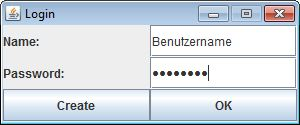
\includegraphics[width=0.4\linewidth]{Login.jpg}
	\captionof{figure}{\small Login}
	\label{Login}
\end{minipage}
\\\\Bei jedem Systemstart öffnet sich ein PopUp-Fenster mit einer Eingabemaske für die Benutzerauthentifizierung. Existiert der eingegebene Benutzer nicht oder ist das zugehörige Passwort falsch, wird das Login-Fenster neu geladen. Mit Create kann ein neuer Benutzer angelegt werden. Desweiteren muss der Anwender das Bucket, auf dem er arbeiten möchte, eintragen. Der Authentifizierungsvorgang beginnt durch Bestätigung von OK.

\textbf{Account erstellen}
\vspace{1em}
$\;$\\
\begin{minipage}{\linewidth}
	\centering
	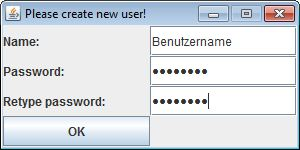
\includegraphics[width=0.4\linewidth]{Create.jpg}
	\captionof{figure}{\small Account erstellen}
	\label{Create}
\end{minipage}
\\\\Durch betätigen der Create-Auswahl im Login-Fenster öffnet sich ein weiteres PopUp, in dem ein Benutzer angelegt werden kann. Hierfür ist ein eindeutiger Benutzername, ein Passwort und eine Bestätigung des Passwortes notwendig. Entsprechen alle eingegebenen Daten den Anforderungen, wird nach Bestätigung von OK ein neuer Benutzer erzeugt. Anschließend kann mit diesen Daten der Login im Login-Fenster erfolgen.

\textbf{Hauptfenster}
\vspace{1em}
$\;$\\
\begin{minipage}{\linewidth}
	\centering
	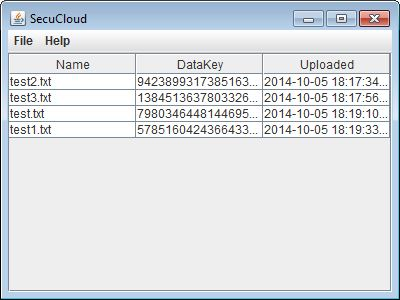
\includegraphics[width=0.4\linewidth]{Main.jpg}
	\captionof{figure}{\small Hauptfenster}
	\label{Main}
\end{minipage}
\\\\Das Hauptfenster zeigt in einer Tabelle die aktuell verfügbaren Daten mit dem Originalnamen, dem zugehörigen verschlüsselten Dateinamen und dem Zeitpunkt des Hochladevorgangs. In der oberen Menüleiste kann das zusätzliche DropDown-Menü File und Help ausgewählt werden. Durch Auswählen einer Zeile mit der linken und Betätigen der rechten Maustaste wird ein Kontextmenü mit Möglichkeiten für diese Zeile/Datei angezeigt.

\textbf{File Menü}
\vspace{1em}
$\;$\\
\begin{minipage}{\linewidth}
	\centering
	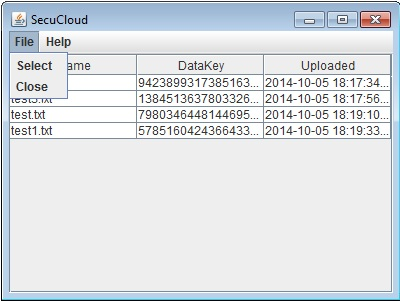
\includegraphics[width=0.4\linewidth]{File.jpg}
	\captionof{figure}{\small File Menü}
	\label{File}
\end{minipage}
\\\\Der Reiter File in der oberen Menüleiste beinhaltet die Auswahlmöglichkeiten Select und Close. Durch Select kann eine lokale Datei zum Verschlüsseln und Upload in die Cloud ausgewählt werden. Close schließt die Anwendung. Die Anzeige der Möglichkeiten kann durch einen Klick auf eine freie Fläche innerhalb der Anwendung oder einen beliebigen Klick in die Oberfläche des Betriebssystems geschlossen werden.

\textbf{Dateiauswahl}
\vspace{1em}
$\;$\\
\begin{minipage}{\linewidth}
	\centering
	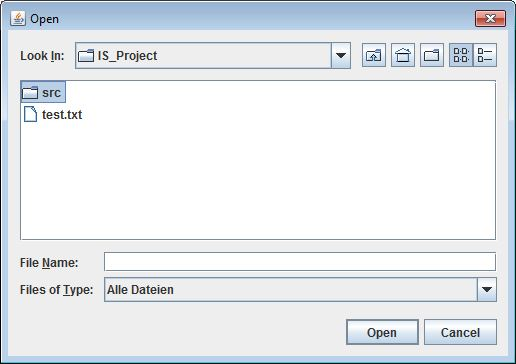
\includegraphics[width=0.4\linewidth]{Select.jpg}
	\captionof{figure}{\small Dateiauswahl}
	\label{Select}
\end{minipage}
\\\\In der Dateiauswahl Select wird die lokale Ordnerstruktur des Betriebssystems angezeigt. In dieser kann sich der Benutzer frei bewegen und in das Quellverzeichnis von Dateien wechseln. Das Auswählen einer Datei und die Bestätigung mit Öffnen initialisiert den, für den Anwender nicht ersichtlichen, Verschlüsselungsvorgang und Dateiupload. Das Auswahlfenster wird beendet. Wurde die Datei korrekt verschlüsselt und in die Cloud geladen, wird diese im Hauptfenster mit ihren Merkmalen aufgelistet. Bei großen Dateien kann dieser Vorgang eine längere Zeitdauer in Anspruch nehmen. Schließt der Benutzer die gesamte Anwendung vor Auflistung in der Dateiübersicht, so wird diese weiterhin durch Hintergrundprozesse verschlüsselt bzw. hochgeladen. Durch Abbrechen kann das Auswahlfenster für Dateien geschlossen werden.

\textbf{Help Menü}
\vspace{1em}
$\;$\\
\begin{minipage}{\linewidth}
	\centering
	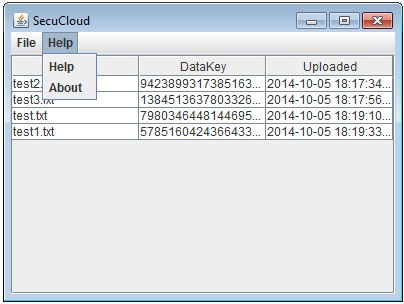
\includegraphics[width=0.4\linewidth]{Help.jpg}
	\captionof{figure}{\small Help Menü}
	\label{Help}
\end{minipage}
\\\\Der Reiter Help in der oberen Menüleiste beinhaltet die Auswahlmöglichkeiten Help und About. Die Auswahl Help öffnet ein zustäzliches Fenster mit Hilfestellungen zur Verwendung, About ein weiteres mit Informationen zu der Software. Die Anzeige der Möglichkeiten kann durch einen Klick auf eine freie Fläche innerhalb der Anwendung oder einen beliebigen Klick in die Oberfläche des Betriebssystems geschlossen werden.

\textbf{Help Fenster}
\vspace{1em}
$\;$\\
\begin{minipage}{\linewidth}
	\centering
	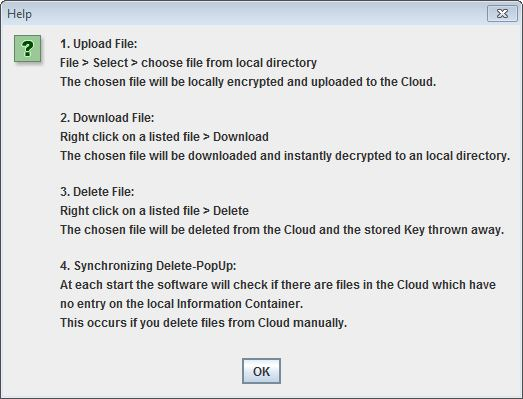
\includegraphics[width=0.4\linewidth]{HelpPopUp.jpg}
	\captionof{figure}{\small Help Fenster}
	\label{HelpPopUp}
\end{minipage}
\\\\Das Help Fenster beschreibt alle Funktionalitäten der Software sowie deren Aufrufe. Mit der Bestätigung von OK wird dieses  geschlossen.

\textbf{About Fenster}
\vspace{1em}
$\;$\\
\begin{minipage}{\linewidth}
	\centering
	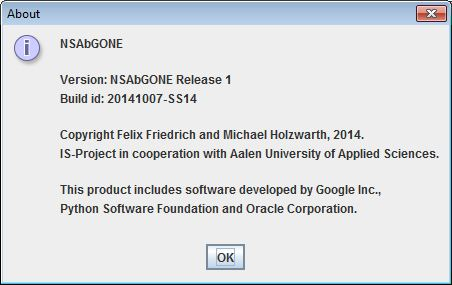
\includegraphics[width=0.4\linewidth]{AboutPopUp.jpg}
	\captionof{figure}{\small About Fenster}
	\label{AboutPopUp}
\end{minipage}
\\\\Das About Fenster gibt Informationen über die Version, Entwickler, den Hintergrund der Entwicklung und Einsatz von Drittanbieter-Software wieder. Durch OK wird geschlossen.

\textbf{Kontextmenü}
\vspace{1em}
$\;$\\
\begin{minipage}{\linewidth}
	\centering
	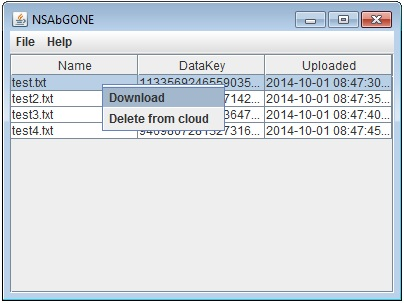
\includegraphics[width=0.4\linewidth]{Kontext.jpg}
	\captionof{figure}{\small Kontextmenü}
	\label{Kontext}
\end{minipage}
\\\\Das Kontextmenü wird durch Auswahl einer Zeile und Betätigen der rechten Maustaste ausgeführt. Es beinhaltet die Möglichkeiten Download und Delete from Cloud. Download initialisiert das temporäre Herunterladen der ausgewählten Datei mit anschließender Entschlüsselung und entschlüsselter Ablage in HOME/SecuCloud/\textless Benutzername\textgreater/download. Mit Delete from Cloud kann eine Datei aus der Cloud zusammen mit dem zugehörigem lokal gespeicherten Schlüssel gelöscht werden. Der Eintrag wird anschließend aus der Dateiübersicht entfernt. Das Kontextmenü kann durch einen Klick auf eine freie Fläche innerhalb der Anwendung oder einen beliebigen Klick in die Oberfläche des Betriebssystems geschlossen werden.

\textbf{Synchronisierungsstatus}
\vspace{1em}
$\;$\\
\begin{minipage}{\linewidth}
	\centering
	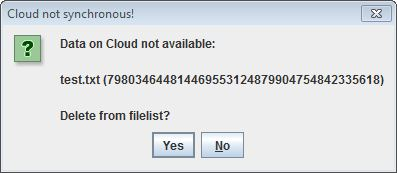
\includegraphics[width=0.4\linewidth]{Synchron.jpg}
	\captionof{figure}{\small Synchronisierungsstatus}
	\label{Synchron}
\end{minipage}
\\\\Das Fenster über den Synchronisierungsstatus kann vom Anwender selbst nicht geöffnet werden. Es erscheint beim Start der Software nur dann, wenn ein lokaler Eintrag einer Datei (mit zugehörigem für den Benutzer nicht ersichtlichen Schlüssel) existiert, diese sich aber nicht mehr in der Cloud befindet. Beispiel für das Hervorrufen eines solchen Ereignisses ist das manuelle Löschen von Dateien in der Cloud-Umgebung. Durch Yes wird der Eintrag in der Dateiübersicht und Datenverwaltung der Software gelöscht. Ein Betätigen von No beendet das Fenster bis zum nächsten Start der Software ohne Ausführen von Aktionen.
\pagebreak

% ----------------------------------------------------------------------------------------------------------
% Diskussion
% ----------------------------------------------------------------------------------------------------------
\section{Diskussion}
Im folgenden Kapitel werden die Ergebnisse der Projektarbeit in der aktuellen Lage (NSA, Prism etc.) eingeordnet. Außerdem wird auf mögliche Erweiterungen der Applikation, sowie weitere mögliche Konzepte der verschlüsselten Datensicherung in der Cloud, eingegangen. 

\subsection{Bedeutung}
Dass Cloud Computing in der heutigen Zeit eine immer größere Bedeutung zukommt und es durchaus auch seine Existenzberechtigung im Sinne von ökonomischen und ökologischen Gesichtspunkten hat soll hier nicht weiter thematisiert werden, da es in \ref{CloudV} Daseinsberechtigung Cloud Computing ausführlich dargelegt wurde. Das essentielle Problem beim Cloud Computing, dass die meisten Anbieter im Ausland liegen und damit nicht unter deutsches Recht fallen, macht es jedoch für viele Anwendungen unbrauchbar. Auf der einen Seite ist der Datenschutz nicht gewährleistet, was grade bei den empfindlichen deutschen Datenschutzgesetzen gefährlich sein kann. Auf der anderen Seite haben die Enthüllungen der letzten Monate gezeigt, dass sogar auf staatlicher Ebene massiv Industriespionage betrieben wird. Dies ist für die meisten deutschen Firmen, die sich ob des hohen Lohnstandards nur aufgrund von technischem Know-How und moderenen Entwicklungen gegen Konkurrenten aus dem Ausland durchsetzen können, ein ausreichender Grund, Cloud Computing zu meiden. Diese Umstände werden durch Applikationen wie der, die im Rahmen dieses Projektes prototypisch entwickelt wurde, behoben. Durch die vorverschlüsselte Ablage muss die genutzte Infrastruktur nicht mehr als sicher angesehenund kann ohne Vorbehalte in dieser Hinsicht genutzt werden. Sehr bewusst wurde bei der Konzeptionierung darauf geachtet, auch BSI Standards für die Verschlüsselung abzudecken. Weniger weil es keine weiteren guten Verschlüsselungssysteme gäbe, als vielmehr um dem deutschen Datenschutz gerecht zu werden, und zu zeigen, dass es durchaus möglich ist, im Ausland Daten derart abzusichern, dass sie als sicher im Sinne der deutschen Gesetzgebung gelten.

\subsection{Erweiterung der Funktionalitäten}
Im folgenden werden Möglichkeiten beschrieben, die bestehende Applikation zu verbessern, ohne dass dazu die grundlegende Architektur verändert werden muss. TODO
\subsubsection{Erhöhung der Bedienerfreundlichkeit}
\textbf{Ausbau des Designs/Multirow}\\
Eine sehr simple, aber dennoch äußerst nützliche Erweiterung des bestehenden Tools wäre es zu ermöglichen, dass ein Anwender mehrere Zeilen der Tabelle markieren und bearbeiten kann. Dies würde die intuitive Nutzbarkeit erhöhen und den Umgang mit großen Dateimengen erleichtern. 
\\\textbf{Drag\&Drop}\\
Um die Benutzerfreundlichkeit des Programmes zu erhöhen wäre es vorteilhaft, Dateien per Drag\&Drop in das Programmfenster hinen zu ziehen. Dadurch müsste ein Benutzer nicht jedes mal, wenn er eine Datei hinzufügen möchte, durch die Verzeichnisstruktur seines Betriebssystems navigieren.
\\\textbf{Autokonfiguration der Schnittstellen}\\
Zurzeit muss gsutil noch manuell vorkonfiguriert werden, um es anschließend mit der Software als Schnittstelle zu Google Cloud Storage zu verwenden. Diese Konfiguartion könnte automatisiert durch die Software selbst geschehen.
\\\textbf{Installations Setup}\\
Die gesamte Installation des Programmes kann durch einen Wizard derart automatisiert werden, dass auch Zusatzsoftware wie Python installiert und die Pfade in Konfigurationsdateien hinterlegt werden. Auch wäre es möglich Python für Windowssysteme automatisch bereit zu stellen und in der .jar Datei zu verpacken. Linux und MAC Systeme besitzen ohnehin standardmäßig eine Python2x Installation und verwenden Standardpfade für installierte Anwendungen (/bin, /usr/bin etc.).
\\\textbf{Selbstsynchronisierung}\\
Um weitere Verwendungsfelder für die Applikation zu erschließen, ist es sinnvoll die in der Cloud hinterlegten Dateien selbstsynchron mit ihren lokalen Pendants zu halten: Jedes Mal, wenn indizierte Dateien geändert werden, berechnet die Applikation ein Changeset der alten und der neuen Version und legt auch dieses verschlüsselt in der Cloud ab. Durch eine neue Ansicht kann der Anwender dann durch Versionen gehen und alte nach Bedarf wieder herstellen. Dadurch wäre eine Art Backupsystem geschaffen, dass nicht nur Sicherheit gewährleistet, sondern gleichzeitig auch Redundanz und Hochverfügbarkeit für die versionierten Daten geschaffen wird.
\\\textbf{Virtuelles Laufwerk/Synchrone Dateistrukturen}\\
Weiterhin denkbar wäre, die Applikation derart anzulegen, dass sie den Cloudspeicher als virtuelles Laufwerk im System verankert. Daten die darin abgelegt werden, werden on the fly verschlüsselt und in der Cloud gespeichert. Dies könnte auch mittels eines automatisch synchronisierten Ordners geschehen, wie es etwa bei Dropbox der Fall ist. Es ergäbe sich allerdings das Problem, dass es Automatismen geben müsste, die verhindern, dass Daten verloren gehen, wenn der synchrone Ordner auf mehreren Systemen gelichzeitig genutzt würde und zwei Personen zur selben Zeit an der selben Datei arbeiten. Hier wäre eine Art Versionsverwaltung von Nöten, die ähnlich wie GIT Changesets von den Dateien erzeugt und diese Verfügbar hält.
\\\textbf{Verschlüsselung von Dateistrukturen}\\
Im Rahmen der zur Verfügung stehenden Zeit für die Bearbeitung der Projektarbeit, wurde eine Verschlüsselung auf dem Datei-Level gewählt. Dies bedeutet, dass gezielt einzelne Dateien zur Verschlüsselung ausgewählt werden können. Ein Kryptosystem wäre jedoch auch für den Einsatz auf weiteren Leveln möglich. Hierzu gehört die Verschlüsselung auf dem Datenträger-Level, d.h. das gesamte Betriebssystem inklusive der beinhaltenden Anwendungen und Daten werden auf einem verschlüsselten Datenträger abgelegt. Dies führt jedoch zu starken Einbußen der Performance und Zuverlässigkeit. Ein weiteres Level bildet das Dateisystem. In diesem werden komplette Verzeichnisse als Container ver- und entschlüsselt. Dieser Anwendungsfall bietet zudem die Möglichkeiten Daten nach ihrer Sensibilität einzustufen und jeweils in ihrer Gesamtheit mit einem eigenen Schlüssel zu versehen. Das letzte Level stellt das Anwendungs-Level dar. Darin verwaltet eine Anwendung die Ver- und Entschlüsselung von Daten. \cite{38}
\\\textbf{Schutz der .boto}\\
TODO

\subsubsection{Serverseitiges Management}
Die folgenden Abschnitte sind kaum mit Quellen versehen, da sie aus eigenen Gedanken entstanden sind. Sollte es ähnliche Verfahrensweisen in anderen Systemen geben, so ist dies Zufall und bedeutet nicht, dass Quellen vorsätzlich unterschlagen wurden.\\
\textbf{Schlüsselmanagement durch Key-Server}\\
Ein potentieller Einsatz der Software auf mehreren Endgeräten macht zwangsläufig ein serverseitiges Schlüsselmanagement unabdingbar. Hinzu kommt eine lange Rückhaltezeit der Schlüssel für verschlüsselt abgelegte Dateien. Dies verringert weniger die Anzahl von abzusichernden Geheimnissen, es verringert lediglich deren Größe (Schlüsselgröße meist kleiner als Dateigröße). TODO \cite{38}
\\\textbf{Loginserver}\\
Um die Applikation unabhängiger von einem bestimmten Cloudanbieter zu halten, wäre ein Konzept mittels Loginserver sinnvoll: Ein Benutzer hat einen Account bei diesem und meldet sich bei Programmstart an. Möchte er eine Datei hochladen, fragt er beim Loginserver an, wohin dies geschehen soll und dieser antwortet mit einem Cloudverzeichnis. Ebenso geschieht es beim Herunterladen der Daten. Möchte der Betrieber des Systems nun einen anderen Cloudanbieter nutzen, etwa weil dieser ein besseres Angebot unterbeitet hat, zieht er alle Daten um und hinterlegt dies beim Loginserver. Der Benutzer merkt von dieser Änderung nichts, aber das Programm arbeitet nun auf einem anderen Speicher als zuvor. Außerdem könnte so auch eine Rechteverwaltung gestaltet werden, sodass der Loginserver den Cloudspeicher verwaltet und den Benuzern selbstständig nur dort Rechte auf dem Speicher gibt, wo sie welche haben sollen und jedes mal neue, wenn sie neue Daten ablegen wollen.
\\\textbf{Providing Server}\label{provV}\\
Die Tatsache, dass Benutzer zurzeit auf dem selben Cloudspeicher arbeiten und eventuell sogar die selben Buckets nutzen, verursacht zwei grundsätzliche Probleme: Zum Einen kann ein Benutzer theoretisch (wenn auch nicht mit der Applikation selbst, aber mittels des Webfrontends) Daten anderer Nutzer manipulieren oder löschen. Dieses Problem ließe sich durch die von den Cloudanbietern selbst angebotene Rechteverwaltung innerhalb des Speichers lösen. Auf der anderen Seite ist es aber dem Cloudanbieter noch möglich einzusehen, welchem Nutzer welche Dateien zuzuordnen sind, was widerum eine Gefahr im Sinne der IT-Sicherheit darstellt: Der Anbieter (oder jede Person oder Organisation die sich auf irgendeine Weise Zugriff verschafft hat) kann Analysen über das Uploadverhalten anfertigen und dadurch Schlüsse auf den Inhalt der Daten ziehen. An dieser Stelle könnte man über den Einsatz eines providing Servers nachdenken: Dieser Server steht zwischen dem Endanwender und dem Cloudspeicher selbst. Alle Daten werden weiterhin lokal verschlüsselt, aber nicht direkt in der Cloud abgelegt, sondern an den providing Server gesendet, welcher sie anschließend auf den oder die Cloudspeicher legt und eine Abbildung der Zugehörigkeiten speichert. Dadurch bleiben die Daten sicher verschlüsselt und und für einen Dritten nicht ersichtlich. Allerdings sind die Daten aus Sicht des Cloudanbieters der selben Person zuzuordnen und jeder der sich unrechtmäßig oder auch rechtmäßig Zugriff zu der Cloud verschaffen kann, ist nicht in der Lage sie zuzuornen. Sollte sich eine Person oder Organisation Zugriff auf den providing Server verschaffen, kann sie zwar Einsicht in die Zuordnung nehmen, aber sie dennoch nicht entschlüsseln. Ein potentieller Angreifer muss also zwei Server überwinden um die obenen genannten Analysen anzufertigen. Im Sinne der aktuellen Enthüllungen über Geheimdienste und Polizeiorganisationen in den USA aber auch dem Rest der Welt wäre hier durchaus Sinnvoll zwar einen der großen (und daher billigen) Cloudanbieter der USA zu wählen, die providing Server aber national zu halten. Solange man der eigenen Nation mehr traut als den USA, wurde hier Sicherheit gewonnen. Alternativ könnte für den providing Server auch ein Standort gewählt werden, der sich in einem Land befindet, welches politisch diametral zu den westlichen Industrienationen steht. Dass es einem Geheimdienst möglich ist, durch rechtmäßige Verfahren Zugriff auf beide Datenpools zu erhalten wird so sehr unwahrscheinlich und erhöht deren Aufwand weiter.
\\\textbf{Serverseitige Rechteverwaltung/Teilen von Dateien}\\
Sollte es einen obig genannten providing Server geben, ist stellt die Rechteverwaltung kein Problem dar: Der Server verwaltet die Accounts der Nutzer und sorgt dafür, dass er zwischengeschaltet ist, dass Nutzer nur an Dateien kommen, die ihnen auch gehören bzw. für die sie Rechte von anderen Nutzern erhalten haben. Diese Berechtigungen können vergeben werden indem die Nutzer einander die Schlüssel zukommen lassen und dem Server mitteilen, dass ein weiterer Nutzer Zugriff bekommen soll. Der Schlüsselaustausch darf hier keinesfalls über den login/providing Server geschehen, da dies dafür sorgen würde, dass Dritte uneingeschränkt Dateien lesen können (nämlich der Betreiber des Loginservers). Alternativ könnten die Schlüssel über den Server verteilt werden, dann allerdings wieder mit einer asymmetrischen Chiffre verschlüsselt. Wichtig ist hierbei, dass der Austausch der asymmetrischen Schlüssel sicher erfolgt um Man-In-The-Middle Angriffe zu verhindern. Eine Orientierung an den Schlüsselservern des PGP Projektes ist hier sinnvoll.

\subsubsection{Erweiterte Sicherheit}
Im folgenden Abschnitt werden Methoden beschrieben, welche die Sicherheit des Systems weiter erhöhen können oder durch alternative Sicherheitsmechanismen die Anwendungsbreite der Applikation erhöhen.
\\\textbf{OpenJDK}\\
Im Laufe der Projektarbeit kamen seitens des betreuenden Professors Zweifel auf, ob die Wahl von Java als Plattform und Programmiersprache sinnvoll war, da Java als nicht besonders sicher gilt. Grundsätzlich sollte die Sicherheit von Java in diesem Projekt keine Rolle spielen, da der Rechner auf dem die Applikation läuft, als sicher gilt und die erzeugten Chiffrate überprüfbar korrekt nach den NIST Standards sind. Trotzdem sorgt die Verwendung von Java in diesem Bereich auf der einen Seite für einen bitteren Beigeschmack und außerdem gibt es eine OpenSource Implementierung die als sicherer gilt: OpenJDK. Das Projekt wurde sowohl unter Windows und dem Oracle Java als auch unter Linux und OpenJDK entwickelt und getestet. Dies stellt also eine mögliche Alternative dar und kann bei der Kompilation wie auch beim Betrieb der Applikation ohne Einschränkung verwendet werden. 
\\\textbf{Alternative Programmiersprachen}\\
Im Rahmen der Überlegungen zu Java und OpenJDK kamen auch Vorschläge zu alternativen Programmiersprachen auf. Hier bietet sich vor allem C++ an, da es für alle gängigen Plattformen Compiler gibt, es strikt objektorientiert ist und sehr exakten Zugriff auf den Speicher zulässt, was zur Absicherung der Schlüssel auf dem Hostsystem wertvoll ist. Hier erhöht sich zwar der Enwicklungsaufwand (siehe \ref{JavaV} Java), dafür kann die Applikation auf dem Hostsystem besser abgesichert werden. So wird ein Betrieb auf Fremdsystemen, zum Beispiel von einem USB Stick aus, noch interessanter.
\\\textbf{Kaskadierte Verschlüsselung}\\
Zwischenzeitlich gab es Überlegungen dahingehend, dass aus der Applikation eine Art Teamplattform mit Versionsverwaltung zu schaffen. Alleine die Berechnung und Verwaltung der Changesets hätte den Rahmen dieser Projektarbeit gesprengt, allerdings kam in diesem Zusammenhang die Idee auf, Verschlüsselungskaskaden aufzubauen um Rechte derart abzubilden, wie sie in Organisationsstrukturen vorkommen: Eine Person steht auf einer bestimmten Stufe und ist berechtigt alles zu sehen/betreten/wissen, was von seiner Sicherheitseinstufung gleichwertig oder niedriger steht.
In diesem Falle ist eine asymmetrische Chiffre unabdingbar. Die Daten werden zunächst wie gehabt verschlüsselt, die Schlüssel allerdings direkt mit abgelegt. Bevor dies geschieht werden sie asymmetrisch mit einer Art Metaschlüssel (dem öffentlichen an dieser Stelle) chiffriert. Dieser ist Teil des Ebenenschlüssels zu der die Datei gehört. Die Ebenenschlüssel sind keine reinen Schlüssel im eigentlichen Sinne, sondern ein Schlüsselpaket, welches alle asymmetrischen privaten Schlüssel umfasst, welche den darunter liegenden Ebenen zugeordnet sind. Die öffentlichen Schlüssel sind allesamt frei zugänglich. Jetzt ist es möglich einer Person Rechte auf einer bestimmten Kaskade zuzuordnen und ihr damit auch Zugriff auf die darunter liegenden zu geben. Eine Person die in einer tieferen Ebene steht kann aber Daten für höhere Ebenen ablegen, wodurch sie selbst eigentlich nicht mehr an die eigene Datei heran kommt, es sei denn sie behält den symmetrischen Schlüssel selbst.

Gedacht war die Umsetzung und Nutzung derart: Ein Unternehmen, nehmen wir hier mal als Beispiel ein Architekturbüro, arbeitet, um die Vorteile von Cloudspeichern zu nutzen und um den Mitarbeitern Unterwegs zugriff auf die Daten zu gewähren, anstatt auf firmeninternen Ablagen direkt auf einem Cloudspeicher. Jeder Architekt erhält nun den Ebenenschlüssel der Ebene, der er zugeordnet ist und kann durch sein Interface auf alle Daten direkt zugreifen. Ob von einem Laptop, dem Büro oder dem Smartphone spielt hier keine Rolle. Steigt er eine Ebene auf oder ab erhält er entsprechend den neuen Ebenenschlüssel. Damit ein findiger Architekt nicht hingehen kann, und sein Ebenenschlüssel speichert, bevor er hinabgestuft wird, werden die symmetrischen Schlüssel jede Nacht neu asymmetrisch verschlüsselt und die Firma betriebt einen eigenen kleinen Server der diese neuen Ebenenschlüssel erzeugt und anhand der Berechtigungen verteilt. Ausserdem kann einem entlassenen Mitarbeiter auch der gesamte Zugriff auf den Cloudspeicher verwehrt werden, sodass er mit seinen (noch gültigen) Schlüsseln nichts mehr anfangen kann.
\\\textbf{Key recovery/Masterkey}\\
Bei allen Vorteilen die ein System mit lokaler Verschlüsselung bietet, entsteht auch immer ein Nachteil: Sollte der Nutzer (oder Kunde) seine(n) Schlüssel verlieren, sind alle gespeicherten Daten verloren sofern das System richtig arbeitet. Eine Lösung dieses Problems, die die Sicherheit zwar schmälert, aber dritten keinen Einblick in die Daten gewährt soll in diesem Abschnitt vorgestellt werden.

Voraussetzung für diese Möglichkeit ist ein System, bei dem der Nutzer seine Daten symmertrisch verschlüsselt und auch die Abbildungstabelle (Schlüssel und Zuordung zu Dateien) asymmetrisch chiffriert in der Cloud ablegt, wie es zum Beispiel in \ref{provV} beschrieben wird. In diesem Fall hat der Nutzer mit dem privaten asymmetrischen Schlüssel eine Art Masterkey, mit dem auf die Gesamtheit seiner Daten zugegriffen werden kann. Die Idee ist nun, diesen Masterkey zu einem Shared-Secret wie es zum Beispiel von Adi Shamir vorgeschlagen wurde, zu machen. Der Nutzer generiert also selbststänfig (dies ist wichtig für die Vertraulichkeit!) aus seinem Masterkey zwei Gehemnisse, die nur gemeinsam eine Wiederherstellung des Schlüssels erlauben. Den einen Teil behält er selbst. Dieser kann bei einer vertrauenswürdigen Person hinterlegt werden, im Tresor einer Bank etc.. Den zweiten Teil gibt er an eine Instanz ab, bei der er mit seinen Personalien registriert ist (erhöhte sicherheit: Biometrische Verfahren). Im Falle eines Gschäftsmodells ist dies die Firma, die den Service anbietet. Verliert der Nutzer seinen Schlüssel, ist es möglich mittels der beiden Geheimnisse seinen Masterkey erneut zu erzeugen. Gleichzeitig kann aber die Instanz mit dem zweiten Teilschlüssel alleine nichts anfangen und auch der Besitzer des ersten Teils kann sich selbstständig keine Zugriff auf die Daten verschaffen.\cite{11}
\\\textbf{Fraktionierung}\\
Einer effektivsten Ansatzpunkte die ein Angriff auf die Verschlüsselung zurzeit hat, ist eine Analyse der Dateigrößen und damit verbundene Rückschlüsse auf deren Inhalt. Dies ist nicht nur gefährlich weil solche Informationen manchem Angreifer schon ausreichen, sondern auch, weil darüber Vermutungen über den Dateityp angestellt werden können. Dies wiederum bedeutet, dass Teile des Klartextes bekannt sind, da viele Dateitypen teils sehr große Header haben, die sich im Inhalt kaum Unterscheiden. Ein Angriff auf die verschlüsselung hingegen hat sehr viel großere Chancen, wenn Teile des Klartextes bekannt sind. Diese Methode nennt sich Known-Plain-Text Angriff. Um diese Schwachstelle zu entfernen ist es nützlich die Dateien vor der Verschlüsselung zu fraktionieren, also in Teile einer definierten Größe zu zerteilen. Ist eine Datei kleiner als die Blockgröße wird sie aufgefüllt mit später entfernbaren Bytefolgen. Nun liegen im Cloudspeicher unzusammenhängende Bitblöcke die keinerlei auskunft über Dateityp oder Inhalt zulassen. Im Falle eines providing Servers, weiß der Cloudanbieter nichtmal wem welcher Block gehört und der providing Server nicht welche Blöcke des Kunden zusammen gehören und eine Datei bilden, nichtmal in welcher Reihenfolge sie sein sollen. Die Applikation könnte die Blöcke nämlich in zufälliger Rehenfolge verschlüsseln und hochladen.
\\\textbf{Verschlüsselte Container}\\
Manche sicherheitssysteme (zum Beispiel TrueCrypt) arbeiten mit verschlüsselten Containern. Dies bedeutet, dass zunächst festgelegt wird, wie groß die verschlüsselte Datenmenge maximal sein darf. In dieser Größe wird nun eine Datei angelegt, gefüllt mit zufälligen Bits. Wenn der Anwender eine Datei in diesen Container hinen Speichern möchte, verschlüsselt er sie und überschreibt einen Teil der Zufallsbits mit dem Chiffrat. Ein Angreifer der des Containers habhaft wird ist nicht in der Lage zu sagen, ob, wie viel, und wo Dateien in dem Container liegen, was die entschlüsselung beinahe unmöglich macht. Auf das Projekt abgebildet würde dies allerdings einen Vorteil des Cloudspeichers zerstören, nämlich nur so viel Speicher bezahlen zu müssen wie tatscählich gebraucht wird. In einem gewissen Maße bildet aber der Cloudspeicher selbst bei fraktionierung der Daten diesen Vorteil: Der Angreifer sieht Datenfragmente und kann keine Aussage darüber treffen, wo Deteien beginnen oder enden, wieviele es gesamt sind, oder wie groß sie sind.
\\\textbf{Rechteverwaltung}\\
Zurzeit gibt es in derApplikation keinerlei Rechteverwaltung auf dem Cloudspeicher selbst. Dies bedeutet, dass ein Nutzer der Zugriffsrechte auf den Cloudspeicher hat, also die Applikation verwenden kann, theoretisch per Webinterface die Daten anderer Manipulieren kann. Dies muss auf Dauer geändert werden. Entweder ist dies über die interne Rechteverwaltung der Cloudanbieter möglich, oder aber durch Login- und Providing wie sie in TODO beschrieben wurden.Dies kann in der Applikation selbst geschen oder der Cloudspeicher wird manuell dahingehend bearbeitet, wenn neue Nutzer hinzu kommen. Im Falle von Google Cloud Storage wäre es möglich, dass bei neuanlegen eines Nutzers ein für ihn vorgesehener Bucket erstellt wird, auf den (und nur auf den) nur der Nutzer schreibrechte hat. Leserechte sind aufgrund der Verschlüsselung eher unktitisch. Außerdem ist der Hintergrund der Software ja das misstrauen gegenüber dem Cloudanbieter selbst, der ohnehin Schreib- und Leserechte auf alle Dateien besitzt.

\subsection{Geschäftsmodell: Sichere Cloudspeicher}
TODO
\\\textbf{Traffic Überwachung}\\
TODO
\pagebreak


	
% ----------------------------------------------------------------------------------------------------------
% Literatur
% ----------------------------------------------------------------------------------------------------------
 
 \begin{thebibliography}{xxxxxxxxxxxxxxxxxxx}
	\bibitem[Oracle]{1}\url{http://www.oracle.com/technetwork/java/javase/overview/javahistory-index-198355.html}
	\bibitem[WJava]{2}\url{http://de.wikipedia.org/wiki/Java_(Programmiersprache)}
	\bibitem[WJavaTechnology]{3}\url{ http://de.wikipedia.org/wiki/Java-Technologie}
	\bibitem[NistAes]{4}\url{http://csrc.nist.gov/publications/fips/fips197/fips-197.pdf}
	\bibitem[WAes]{5}\url{http://de.wikipedia.org/wiki/Advanced_Encryption_Standard}
	\bibitem[WCounterMode]{6}\url{http://de.wikipedia.org/wiki/Counter_Mode}
	\bibitem[NistCounterMode]{7}\url{http://csrc.nist.gov/publications/nistpubs/800-38a/sp800-38a.pdf}
	\bibitem[WSha]{8}\url{http://de.wikipedia.org/wiki/Secure_Hash_Algorithm}
	\bibitem[WSha2]{9}\url{http://de.wikipedia.org/wiki/SHA-2}
	\bibitem[NistSha2]{10}\url{http://csrc.nist.gov/publications/fips/fips180-4/fips-180-4.pdf}
	\bibitem[SecShW]{11}\url{http://en.wikipedia.org/wiki/Shamir%27s_Secret_Sharing}
	\bibitem[BsiAlg1]{12}\url{http://www.bundesnetzagentur.de/SharedDocs/Downloads/DE/Sachgebiete/QES/Veroeffentlichungen/Algorithmen/2014Algorithmenkatalog.pdf;jsessionid=44761A7B91153744E5BAC51D89FB1FBD?__blob=publicationFile&v=1}
	\bibitem[BsiAlg2]{13}\url{https://www.bsi.bund.de/SharedDocs/Downloads/DE/BSI/Publikationen/TechnischeRichtlinien/TR02102/BSI-TR-02102_pdf.pdf?__blob=publicationFile}
	\bibitem[Gartner]{30}\url{http://www.gartner.com/technology/reprints.do?id=1-1UKQQA6&ct=140528&st=sb}
 	\bibitem[Git]{31}\url{http://git-scm.com/book}
	\bibitem[gsutil]{32}\url{https://cloud.google.com/storage/docs/gsutil}	
	\bibitem[IEEE]{33}\url{http://ieeexplore.ieee.org/xpl/login.jsp?tp=&arnumber=5565955&url=http%3A%2F%2Fieeexplore.ieee.org%2Fxpls%2Fabs_all.jsp%3Farnumber%3D5565955}
	\bibitem[NistCc]{34}\url{http://csrc.nist.gov/publications/nistpubs/800-145/SP800-145.pdf}, S. 2ff.
	\bibitem[BsiCc]{35}\url{https://www.bsi.bund.de/DE/Themen/CloudComputing/Grundlagen/Grundlagen_node.html}
	\bibitem[CsaCc]{36}\url{https://cloudsecurityalliance.org/guidance/csaguide.v3.0.pdf}
	\bibitem[HmdCc]{37}\url{http://link.springer.com/article/10.1007/BF03340515#},  S.77
	\bibitem[Winkler]{38} [Winkler – Securing the Cloud]
	\bibitem[CloudComputing]{39} \url{http://books.google.de/books?hl=de&lr=&id=KJj-0_cPFycC&oi=fnd&pg=PA1&dq=Notwendigkeit+von+Cloud+Computing&ots=O1ppInQq8Q&sig=7CyTpiTQWUIdY8wO__BxgzmXc0I#v=onepage&q&f=false}
	
\end{thebibliography}
\pagebreak

% ----------------------------------------------------------------------------------------------------------
% Anhang
% ----------------------------------------------------------------------------------------------------------
\pagenumbering{Roman}
\setcounter{page}{1}
\lhead{Anhang \thesection}

\begin{appendix}
\section*{Anhang}
\phantomsection
\addcontentsline{toc}{section}{Anhang}
\addtocontents{toc}{\vspace{-0.5em}}

\section{Installationsanleitung}
Detaillierte Beschreibung zum Einsatz auf "Fremdsystemen"
\pagebreak
\section{Digitaler Anhang}
\end{appendix}

\end{document}
